\chapter{Cristalli}

\lezione{14}{14/04/2026}

Le proprietà fisiche dei solidi dipendono dalla composizione e dalla struttura con cui tali componenti si distribuiscono nello spazio occupato dal volume del solido. I componenti o costituenti possono esser atomi, ioni, molecole o complessi la cui interazione mediata da legami chimici può esser più o meno forte e stabile nel tempo.

Osservando le simmetrie presenti in natura, come ad esempio la struttura di un nido d'ape, è possibile notare la presenza di motivi (\textit{pattern}) traslati lungo determinate direzioni, andando a formare geometrie regolari, come degli esagoni.

Cosa hanno in comune queste forme? Definiscono dei materiali solidi caratterizzati da una proprietà fondamentale: la loro struttura si ripete periodicamente nello spazio. Questi materiali prendono il nome di \textbf{cristalli}.

Per descrivere rigorosamente la struttura di un cristallo, è utile separare la geometria del sistema dalla sua composizione materiale. Possiamo infatti definirlo come la combinazione di due entità:
\begin{itemize}
    \item Un \textbf{reticolo} ( in inglese \textit{lattice}): un insieme di nodi, ovvero un costrutto puramente matematico che ne definisce le proprietà geometriche e di simmetria.
    \item Una \textbf{base} (in inglese \textit{basis}): un atomo, uno ione o una molecola (come ad esempio una molecola tetragonale) che va a posizionarsi nel reticolo.
\end{itemize}

In sintesi, un cristallo può essere descritto concettualmente come un insieme di punti nello spazio (il reticolo) a ciascuno dei quali alleghiamo un elemento fisico materiale.


Il reticolo è caratterizzato da una fondamentale invarianza per traslazioni. I \textbf{vettori di traslazione primitivi}, indicati tipicamente con l'insieme \( \{ \vec{a}_1, \vec{a}_2, \vec{a}_3 \} \), fungono da generatori delle traslazioni e devono costituire un set di vettori linearmente indipendenti tra loro.

Questi vettori permettono di coprire e descrivere tutto il cristallo tramite una loro combinazione lineare, definendo così il \textbf{vettore del reticolo cristallino} (o vettore traslazione):
\begin{equation}
    \vec{T} = n_1 \vec{a}_1 + n_2 \vec{a}_2 + n_3 \vec{a}_3
\end{equation}
con i coefficienti \( n_1, n_2, n_3 \in \mathbb{Z} \) e dove la distanza nodo-nodo appartiene all'insieme dei numeri reali (\( \mathbb{R} \)). Grazie a questa formulazione, è possibile descrivere le proprietà dell'intero cristallo guardando e studiando solamente una singola cella, facendo attenzione a rappresentare un'unità che copre bene lo spazio senza contare una stessa porzione due volte.

Al reticolo 3D è associata una \textbf{base}, ovvero un insieme di elementi costitutivi (che possono essere atomi, molecole o complessi). La posizione di questi elementi rispetto a un qualunque punto del reticolo è identificata proprio dalla terna di vettori di base \( \{ \vec{a}_1, \vec{a}_2, \vec{a}_3 \} \). Per "base" si intende quindi non solo l'insieme materiale dei costituenti, ma anche il loro relativo posizionamento spaziale. 

Il reticolo che si riferisce alla struttura che descrive fisicamente il solido cristallino reale prende il nome di \textbf{reticolo diretto}. Come mostrato graficamente, la scelta dei vettori reticolari per descrivere una data disposizione di punti non è univoca: esistono diverse combinazioni di vettori che possono fungere da base per lo stesso luogo di punti.

\begin{figure}[H]
    \centering
    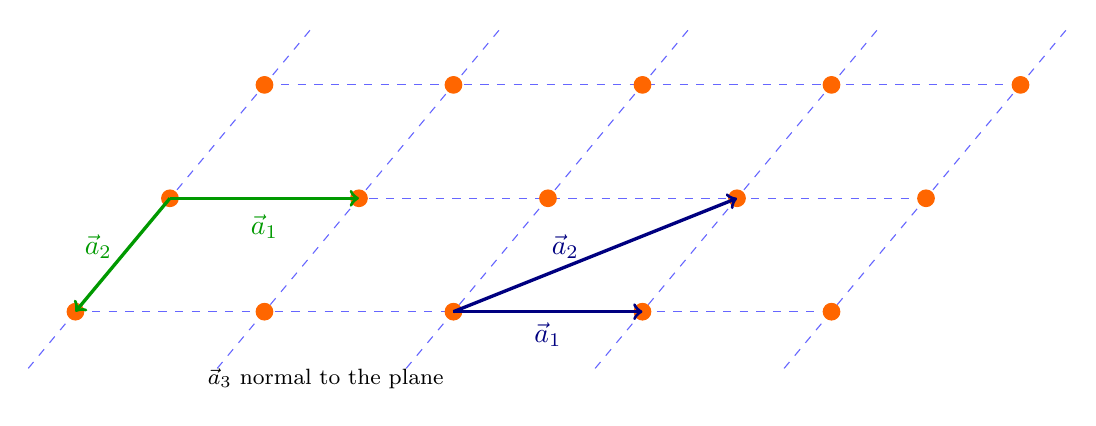
\begin{tikzpicture}[scale=1.2]
        % Definizione dei nodi del reticolo 2D
        \foreach \i in {0, 1, 2, 3,4} {
            \foreach \j in {0, 1, 2} {
                \coordinate (N\i\j) at (-1+\i*2 + \j*1, \j*1.2);
            }
        }
        
        % Linee guida tratteggiate orizzontali (simmetrie)
        \foreach \j in {0, 1, 2} {
            \draw[dashed, blue!60] (-1 + \j*1, \j*1.2) -- (7 + \j*1, \j*1.2);
        }
        % Linee guida tratteggiate diagonali
        \foreach \i in {-1, 0, 1, 2, 3} {
            \draw[dashed, blue!60] (\i*2 + 0.5, -0.6) -- (\i*2 + 3.5, 3);
        }

        % Disegno dei nodi
        \foreach \i in {0, 1, 2, 3,4} {
            \foreach \j in {0, 1, 2} {
                \filldraw[orange!80!red] (N\i\j) circle (2.5pt);
            }
        }

        % Prima scelta di vettori base (Blu)
        \draw[->, very thick, blue!50!black] (N20) -- (N30) node[midway, below] {\(\vec{a}_1\)};
        \draw[->, very thick, blue!50!black] (N20) -- (N31) node[midway, left=2pt, yshift = 3pt] {\(\vec{a}_2\)};

        % Seconda scelta di vettori base (Verdi)
  
        \draw[->, very thick, green!60!black] (N01) -- (N11) node[midway, below=2pt] {\(\vec{a}_1\)};
        \draw[->, very thick, green!60!black] (N01) -- (N00) node[midway, left, yshift = 3pt] {\(\vec{a}_2\)}; 

        % Nota sul vettore normale
        \node[below left, font=\footnotesize] at (3, -0.5) {\(\vec{a}_3\) normal to the plane};
    \end{tikzpicture}
    \caption{Rappresentazione di un reticolo con invarianza per traslazioni. Sono evidenziate due possibili scelte differenti per i vettori di traslazione primitivi (set blu e set verde), a dimostrazione che la scelta della base non è univoca.}
\end{figure}

\begin{note}{Struttura dei solidi}{ stru}
Per \textbf{struttura} si intende la modalità con cui i costituenti si dispongono nello spazio; laddove tale disposizione manifesti dei motivi ripetitivi, si riconoscono delle proprietà specifiche di simmetria.

\begin{itemize}
    \item \textbf{Solidi Cristallini} \\
        I solidi cristallini sono caratterizzati da un ordine a lungo raggio: è possibile riprodurre l'intero cristallo (idealmente infinitamente esteso) ripetendo una sua porzione elementare, detta \textbf{cella unitaria}, mediante traslazioni. Poiché tale ordine si esplica indefinitamente nelle tre dimensioni, la periodicità spaziale è il presupposto fondamentale per la \textbf{descrizione a bande} dei livelli energetici. 
    \item \textbf{Solidi Policristallini} \\
        Questi materiali manifestano ordine localmente, tipicamente su scala micrometrica, ma non globalmente. L'ordine si presenta in aree limitate definite \textbf{domini} o \textbf{grani}. Domini adiacenti possono avere orientamenti cristallini differenti e i confini tra di essi sono denominati \textbf{bordi di grano}.
    \item \textbf{Solidi Amorfi}\\
        I solidi amorfi sono privi di ordine a lungo raggio. Possono tuttavia manifestare un \textbf{ordine a corto raggio} su scala atomica, ovvero limitatamente a una distanza di pochi \AA.

\end{itemize}




\begin{table}[H]
\centering
\begin{tabular}{lll}
\hline
\textbf{Tipologia} & \textbf{Scala di Ordine} & \textbf{Caratteristiche Principali} \\ \hline
Cristallino & Lungo raggio & Cella unitaria, periodicità 3D, simmetria \\
Policristallino & Locale (micrometrica) & Grani, domini, bordi di grano \\
Amorfo & Corto raggio (\AA) & Disordine globale, ordine atomico locale \\ \hline
\end{tabular}
\end{table}
Noi ci concentremo principalmente sui cristalli.

\end{note}

In un solido cristallino, ogni proprietà fisica \( f \) misurata in una posizione \( \vec{r} \) deve soddisfare una condizione di invarianza rispetto alle traslazioni del reticolo. Questo requisito è noto come \textbf{principio di Neumann} e si formalizza come:
\begin{equation}
    f(\vec{r}) = f(\vec{r} + \vec{R}) \quad \forall \vec{R}
\end{equation}
dove \( \vec{R} \) è un vettore del reticolo.

La \textbf{cella elementare} è la porzione minima che conserva le proprietà di simmetria del cristallo e la cui traslazione lungo i vettori \( \vec{R} \) permette di ricostruire l'intero volume senza sovrapposizioni o vuoti. Se la cella ospita un solo nodo reticolare, viene definita \textbf{unitaria}. Tale regione è delimitata dai vettori \( \vec{a}_1, \vec{a}_2, \vec{a}_3 \) che partono da un nodo preso come origine.

Il volume di questa unità fondamentale si ottiene tramite il valore assoluto del prodotto misto dei vettori base:
\begin{equation}
    V_{\text{cella}} = |\vec{a}_1 \cdot \vec{a}_2 \wedge \vec{a}_3|
\end{equation}

A seconda della configurazione dei vettori base e del numero di nodi contenuti, possiamo distinguere:
\begin{itemize}
    \item \textbf{Cella Cartesiana:} quando i vettori del reticolo \( \{\vec{a}_1, \vec{a}_2, \vec{a}_3\} \) risultano allineati ai versori del sistema di riferimento \( \{\vec{u}_x, \vec{u}_y, \vec{u}_z\} \).
    \item \textbf{Cella Convenzionale:} un'unità che rispetta le simmetrie del sistema ma contiene più di un nodo al suo interno.
    \item \textbf{Cella Primitiva:} la cella elementare a volume minimo; per definizione, contiene esattamente un solo nodo.
\end{itemize}

Per ogni nodo del reticolo è possibile identificare gli \textbf{atomi primi vicini}, ovvero gli elementi costitutivi più prossimi; il loro numero totale è indicato come \textbf{numero di coordinazione}.

Un esempio fondamentale di cella primitiva è la \textbf{cella di Wigner-Seitz}. Essa è definita come il luogo dei punti nello spazio più vicini a un determinato nodo rispetto a qualunque altro nodo del reticolo. La sua costruzione prevede di collegare un nodo ai suoi primi vicini e tracciare i piani ortogonali che passano per il punto medio di ciascun segmento di collegamento. Il poliedro risultante dall'intersezione di questi piani è una cella unitaria a volume minimo che, per costruzione, presenta il nodo esattamente al centro.

\subsection{Reticoli di Bravais}

La teoria dei reticoli di Bravais stabilisce che, nello spazio tridimensionale, è possibile identificare 14 configurazioni topologicamente distinte, organizzate in 7 sistemi cristallini derivanti dai gruppi di simmetria puntuale. Sebbene in natura esista un numero infinito di reticoli teorici, questo insieme minimo di 14 configurazioni è sufficiente a descrivere la struttura di tutti i cristalli conosciuti. In uno spazio bidimensionale, tale varietà si riduce a soli 5 reticoli distinti.

\begin{figure}[htbp]
    \centering
    \includegraphics[width=\textwidth]{figures/bravais.png}
    \caption{I 14 reticoli di Bravais nello spazio tridimensionale.}
    \label{fig:bravais_lattices}
\end{figure}


Ogni reticolo di Bravais in 3D è univocamente definito da tre vettori reticolari \( \vec{a}_1, \vec{a}_2, \vec{a}_3 \). Le loro lunghezze, indicate come \( a, b, c \), e gli angoli compresi \( \alpha, \beta, \gamma \) costituiscono i cosiddetti \textbf{parametri di cella}, i quali ne determinano le dimensioni e l'orientamento spaziale. All'interno di una struttura periodica, ogni nodo posto su un vertice della cella è condiviso da 8 celle adiacenti.

\textbf{Sistemi Cristallini e Relazioni Geometriche} \\
I 7 sistemi si differenziano per i vincoli geometrici imposti ai parametri di cella:
\begin{itemize}
    \item \textbf{Cubico:} \( a = b = c \) e \( \alpha = \beta = \gamma = 90^\circ \). Rappresenta il sistema più comune per i cristalli mono-elementali.
    \item \textbf{Tetragonale:} \( a = b \neq c \) e \( \alpha = \beta = \gamma = 90^\circ \).
    \item \textbf{Ortorombico:} \( a \neq b \neq c \) e \( \alpha = \beta = \gamma = 90^\circ \).
    \item \textbf{Romboedrico (Trigonale):} \( a = b = c \) e \( \alpha = \beta = \gamma \neq 90^\circ \).
    \item \textbf{Esagonale:} \( a = b \neq c \), \( \alpha = \beta = 90^\circ \) e \( \gamma = 120^\circ \).
    \item \textbf{Monoclino:} \( a \neq b \neq c \), \( \alpha = \gamma = 90^\circ \) e \( \beta \neq 90^\circ \).
    \item \textbf{Triclino:} \( a \neq b \neq c \) e \( \alpha \neq \beta \neq \gamma \neq 90^\circ \). È la configurazione meno simmetrica, definita da 6 parametri indipendenti.
\end{itemize}

\textbf{Il Sistema Cubico} \\
Data la sua rilevanza, il sistema cubico viene spesso analizzato attraverso tre varianti:
\begin{itemize}
    \item \textbf{Cubico Semplice (SC):} con nodi posizionati esclusivamente sui vertici. Tale cella elementare è anche unitaria.
    \item \textbf{Cubico a Facce Centrate (FCC):} presenta nodi sui vertici e al centro di ogni faccia. Questa cella elementare non è unitaria in quanto contiene più di un nodo per cella.
    \item \textbf{Cubico a Corpo Centrato (BCC):} possiede nodi sui vertici e un nodo aggiuntivo al centro del volume cubico. Anche in questo caso, la cella elementare non coincide con quella unitaria.
\end{itemize}

La realtà naturale mostra strutture spesso più complesse dei singoli reticoli ideali. Molti cristalli risultano dalla combinazione di più reticoli appartenenti anche a sistemi differenti, tra loro traslati nello spazio (come nel caso della struttura del diamante). Altri materiali, come il \textbf{quarzo} (silice cristallina), presentano strutture non cubiche a causa della diversa natura delle forze e dei legami atomici che ne determinano la stabilità.




\begin{figure}[htbp]
    \centering
    \resizebox{\textwidth}{!}{
        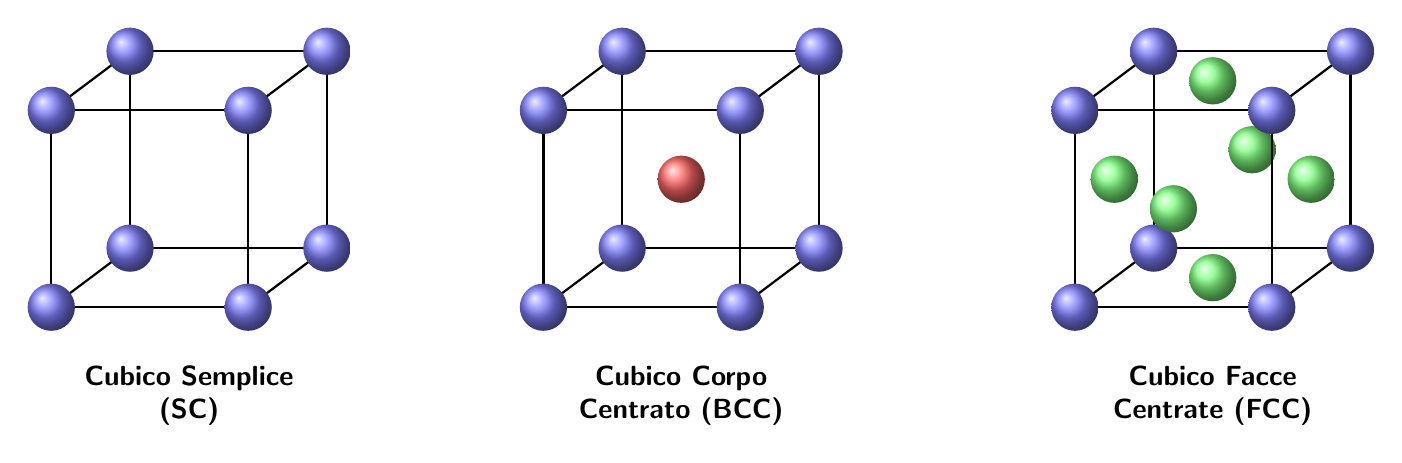
\begin{tikzpicture}[
            % Definizione dell'asse di prospettiva per il 3D
            x={(1cm,0cm)}, y={(0cm,1cm)}, z={(0.4cm,0.3cm)},
            scale=2.5,
            % Stili dei nodi (atomi) e delle linee
            atom/.style={circle, shading=ball, ball color=blue!50, minimum size=0.6cm},
            center_atom/.style={circle, shading=ball, ball color=red!60, minimum size=0.6cm},
            face_atom/.style={circle, shading=ball, ball color=green!50, minimum size=0.6cm},
            edge/.style={thick, line join=round}
        ]

        % ==============================
        % 1. CUBICO SEMPLICE (SC)
        % ==============================
        \begin{scope}[shift={(0,0)}]
            % Spigoli posteriori
            \draw[edge] (0,0,1) -- (1,0,1) -- (1,1,1) -- (0,1,1) -- cycle;
            % Spigoli di connessione (profondità)
            \draw[edge] (0,0,0) -- (0,0,1);
            \draw[edge] (1,0,0) -- (1,0,1);
            \draw[edge] (0,1,0) -- (0,1,1);
            \draw[edge] (1,1,0) -- (1,1,1);

            % Atomi posteriori
            \node[atom] at (0,0,1) {}; \node[atom] at (1,0,1) {};
            \node[atom] at (0,1,1) {}; \node[atom] at (1,1,1) {};

            % Spigoli anteriori
            \draw[edge] (0,0,0) -- (1,0,0) -- (1,1,0) -- (0,1,0) -- cycle;

            % Atomi anteriori
            \node[atom] at (0,0,0) {}; \node[atom] at (1,0,0) {};
            \node[atom] at (0,1,0) {}; \node[atom] at (1,1,0) {};


            % Didascalia
            \node[below=1cm, font=\sffamily\bfseries, align=center] at (0.5,0,0.5) {Cubico Semplice\\(SC)};
        \end{scope}

        % ==============================
        % 2. CUBICO A CORPO CENTRATO (BCC)
        % ==============================
        \begin{scope}[shift={(2.5,0)}]
            % Spigoli posteriori e connessioni
            \draw[edge] (0,0,1) -- (1,0,1) -- (1,1,1) -- (0,1,1) -- cycle;
            \draw[edge] (0,0,0) -- (0,0,1); \draw[edge] (1,0,0) -- (1,0,1);
            \draw[edge] (0,1,0) -- (0,1,1); \draw[edge] (1,1,0) -- (1,1,1);

            % Atomi posteriori
            \node[atom] at (0,0,1) {}; \node[atom] at (1,0,1) {};
            \node[atom] at (0,1,1) {}; \node[atom] at (1,1,1) {};

            % Atomo centrale (Body)
            \node[center_atom] at (0.5,0.5,0.5) {};

            % Spigoli anteriori
            \draw[edge] (0,0,0) -- (1,0,0) -- (1,1,0) -- (0,1,0) -- cycle;

            % Atomi anteriori
            \node[atom] at (0,0,0) {}; \node[atom] at (1,0,0) {};
            \node[atom] at (0,1,0) {}; \node[atom] at (1,1,0) {};

            % Didascalia
            \node[below=1cm, font=\sffamily\bfseries, align=center] at (0.5,0,0.5) {Cubico Corpo\\Centrato (BCC)};
        \end{scope}

        % ==============================
        % 3. CUBICO A FACCE CENTRATE (FCC)
        % ==============================
        \begin{scope}[shift={(5.2,0)}]
            % Spigoli posteriori e connessioni
            \draw[edge] (0,0,1) -- (1,0,1) -- (1,1,1) -- (0,1,1) -- cycle;
            \draw[edge] (0,0,0) -- (0,0,1); \draw[edge] (1,0,0) -- (1,0,1);
            \draw[edge] (0,1,0) -- (0,1,1); \draw[edge] (1,1,0) -- (1,1,1);

            % Atomo sulla faccia posteriore
            \node[face_atom] at (0.5,0.5,1) {};

            % Atomi ai vertici posteriori
            \node[atom] at (0,0,1) {}; \node[atom] at (1,0,1) {};
            \node[atom] at (0,1,1) {}; \node[atom] at (1,1,1) {};

            % Atomi sulle facce laterali, superiore e inferiore
            \node[face_atom] at (0,0.5,0.5) {}; \node[face_atom] at (1,0.5,0.5) {};
            \node[face_atom] at (0.5,1,0.5) {}; \node[face_atom] at (0.5,0,0.5) {};

            % Spigoli anteriori
            \draw[edge] (0,0,0) -- (1,0,0) -- (1,1,0) -- (0,1,0) -- cycle;

            % Atomo sulla faccia anteriore
            \node[face_atom] at (0.5,0.5,0) {};

            % Atomi ai vertici anteriori
            \node[atom] at (0,0,0) {}; \node[atom] at (1,0,0) {};
            \node[atom] at (0,1,0) {}; \node[atom] at (1,1,0) {};

            % Didascalia
            \node[below=1cm, font=\sffamily\bfseries, align=center] at (0.5,0,0.5) {Cubico Facce\\Centrate (FCC)};
        \end{scope}

        \end{tikzpicture}%
    }
    \caption{Rappresentazione dei reticoli cubici: Semplice (SC), a Corpo Centrato (BCC) e a Facce Centrate (FCC).}
    \label{fig:cubic_lattices}
\end{figure}

\subsubsection{Fattore di appartenenza}

Il \textbf{fattore di appartenenza} (o di partecipazione), indicato come \( f_{\text{appartenenza}} \), definisce la frazione di volume di un nodo reticolare che compete effettivamente a una singola cella. All'interno di un reticolo esteso (trascurando gli effetti di bordo), i nodi posizionati sul perimetro della cella sono condivisi tra più celle adiacenti; di conseguenza, il loro contributo volumetrico si ripartisce.

Analizzando il sistema cubico, i fattori di partecipazione assumono i seguenti valori geometrici:
\begin{itemize}
    \item \textbf{Nodo al vertice:} poiché ogni vertice è il punto di incontro di 8 celle cubiche adiacenti, il suo fattore di appartenenza è \( 1/8 \).
    \item \textbf{Nodo al centro della faccia:} essendo localizzato su una superficie di confine condivisa da 2 celle contigue, il suo fattore è \( 1/2 \).
    \item \textbf{Nodo al centro del volume:} trovandosi interamente confinato all'interno della cella, non è condiviso e il suo fattore è pari a \( 1 \).
\end{itemize}

Ipotizzando di disporre un elemento costitutivo (ad esempio un atomo) in ogni nodo, il cristallo risultante sarà descritto da un reticolo e da una base. È possibile calcolare il numero di \textbf{atomi equivalenti} (o nodi netti) che costituiscono la base di una specifica cella cartesiana sommando i contributi frazionari di tutti i suoi nodi.

\textbf{Reticolo Cubico Semplice (SC)} \\
La cella cubica semplice presenta nodi esclusivamente in corrispondenza degli 8 vertici. Il calcolo degli atomi equivalenti è:
\( N = 8 \cdot \frac{1}{8} = 1 \text{ nodo/atomo} \) \\
Poiché contiene un solo nodo netto, la cella cubica semplice è classificata come \textbf{cella unitaria}.

\textbf{Reticolo Cubico a Corpo Centrato (BCC - Body Centered Cube)} \\
Questa configurazione possiede nodi agli 8 vertici e un nodo aggiuntivo al centro geometrico del cubo. Il numero totale di atomi equivalenti risulta:
\( N = \left( 8 \cdot \frac{1}{8} \right) + \left( 1 \cdot 1 \right) = 1 + 1 = 2 \text{ nodi/atomi} \)

\textbf{Reticolo Cubico a Facce Centrate (FCC - Face Centered Cube)} \\
La cella è caratterizzata da nodi agli 8 vertici e un nodo al centro di ciascuna delle 6 facce esterne. Il computo degli atomi equivalenti per cella è:
\( N = \left( 8 \cdot \frac{1}{8} \right) + \left( 6 \cdot \frac{1}{2} \right) = 1 + 3 = 4 \text{ nodi/atomi} \)

\subsubsection{Piani e direzioni cristalline}
Per identificare in modo univoco un piano all'interno di un reticolo, risulta estremamente utile adottare il metodo di indicizzazione proposto da Miller, il quale stabilisce una relazione diretta con la direzione normale al piano stesso. Assegnata una terna di vettori base del reticolo \( \{\vec{a}_1, \vec{a}_2, \vec{a}_3\} \), la procedura operativa per ricavare gli \textbf{Indici di Miller} si articola nei seguenti passaggi:

\begin{figure}[htbp]
    \centering
    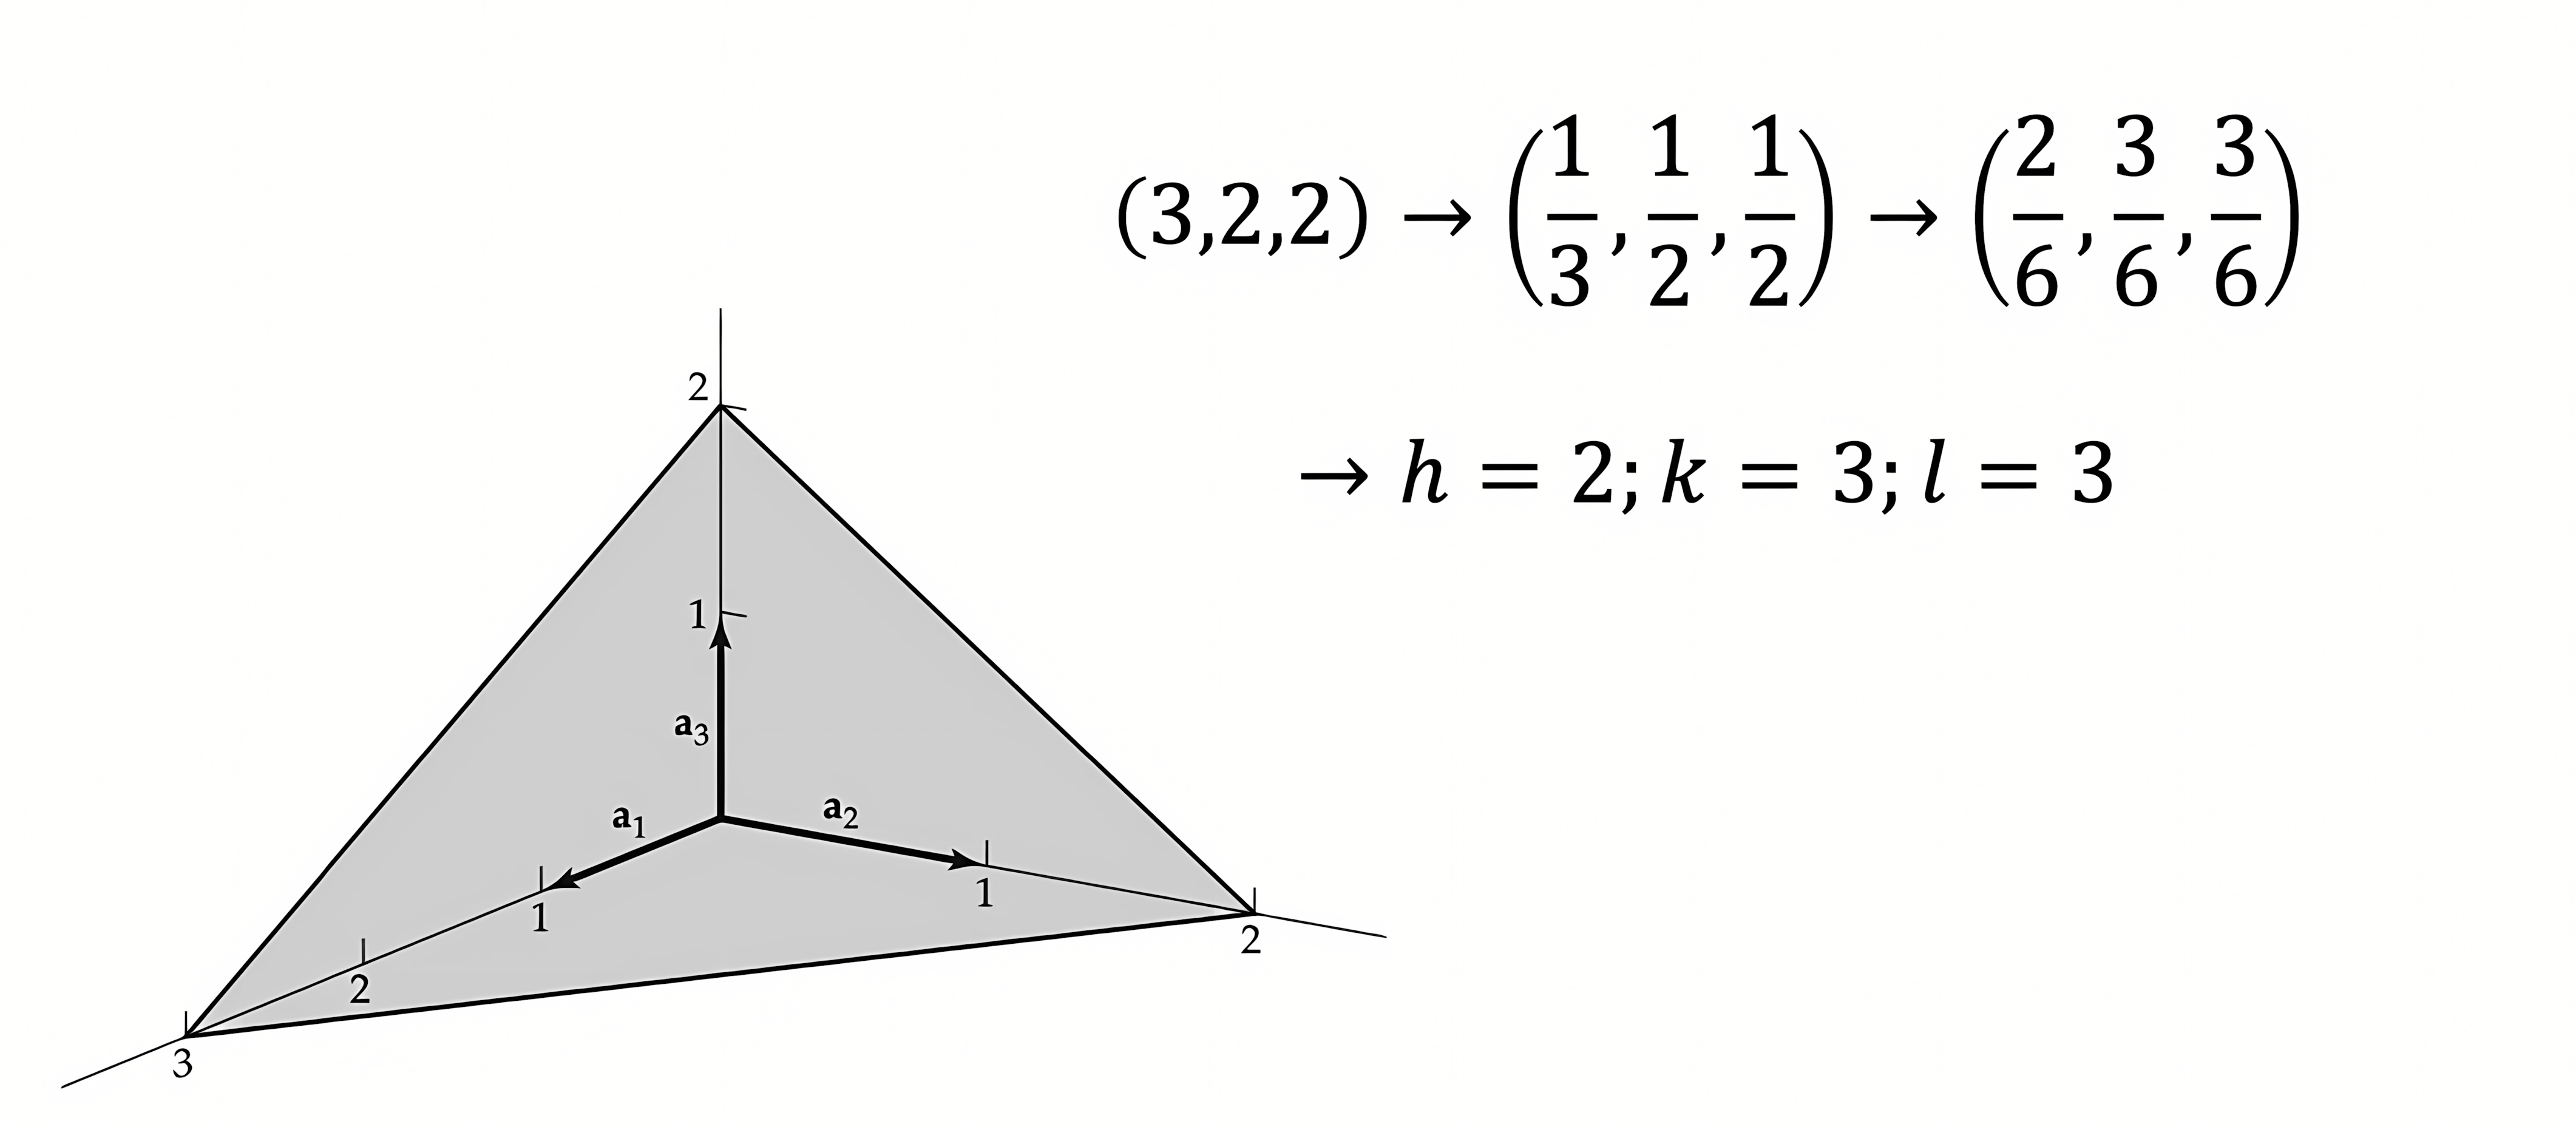
\includegraphics[width=0.8\textwidth]{figures/miller_indices.png}
    \caption{Esempio di piani cristallini e loro indicizzazione tramite indici di Miller.}
    \label{fig:miller_indices}
\end{figure}

\begin{enumerate}
    \item Si determinano i punti di intersezione del piano considerato con gli assi definiti dai vettori base, ricavando così le intercette \( (n_1, n_2, n_3) \).
    \item Si calcolano i reciproci di tali intercette: \( \left( \frac{1}{n_1}, \frac{1}{n_2}, \frac{1}{n_3} \right) \).
    \item Si riducono queste frazioni a un set di numeri interi minimi calcolando il minimo comune multiplo (mcm) dei denominatori. In questo modo si passa a una espressione proporzionale del tipo \( \left( \frac{\text{mcm}}{n_1}, \frac{\text{mcm}}{n_2}, \frac{\text{mcm}}{n_3} \right) \).
    \item Il piano viene infine indicizzato dalla terna racchiusa tra parentesi tonde \( (hkl) \), dove \( h = \frac{\text{mcm}}{n_1} \), \( k = \frac{\text{mcm}}{n_2} \) e \( l = \frac{\text{mcm}}{n_3} \). Tale terna definisce la normale \( \vec{n}_{hkl} \) al piano.
\end{enumerate}



Un esempio pratico: se un piano interseca gli assi in \( (3, 2, 2) \), i rispettivi reciproci sono \( \left( \frac{1}{3}, \frac{1}{2}, \frac{1}{2} \right) \). Moltiplicando per il minimo comune multiplo (pari a 6), si ottengono i valori interi 2, 3 e 3. Il piano sarà quindi indicato come \( (233) \).

L'intero insieme di piani paralleli a quello appena calcolato costituisce una famiglia, la quale viene denotata utilizzando le parentesi graffe: \( \{hkl\} \). Nel caso in cui un indice assuma valore negativo (ad esempio un'intercetta sul semiasse negativo), la convenzione prevede di scrivere una barra al di sopra del numero. Se si considera un reticolo cubico allineato agli assi cartesiani, il piano \( (\bar{1}00) \) è parallelo al piano \( (100) \), ma la sua normale punta nel verso opposto rispetto all'asse \( x \).

\textbf{Direzioni Cristallografiche} \\
Il formalismo si estende anche alle direzioni all'interno del cristallo. Una specifica direzione viene indicata utilizzando le parentesi quadre \( [n_1 n_2 n_3] \) e rappresenta il vettore risultante dalla combinazione lineare \( n_1\vec{a}_1 + n_2\vec{a}_2 + n_3\vec{a}_3 \). Per fare un esempio, la simbologia \( [100] \) identifica esattamente il vettore \( \vec{a}_1 \), mentre \( [\bar{1}00] \) corrisponde al vettore \( -\vec{a}_1 \). Infine, una famiglia che raggruppa tutte le direzioni cristallografiche equivalenti per simmetria viene indicata con le parentesi angolate \( \langle n_1 n_2 n_3 \rangle \).


\subsubsection{Cella primitiva}

Esistono diverse metodologie per identificare una \textbf{cella primitiva}, la quale rappresenta un'unità elementare a volume minimo. La strategia più funzionale prevede l'utilizzo di vettori reticolari che operino contestualmente come vettori di base per il sistema; questi prendono il nome di \textbf{vettori di base primitivi} e vengono indicati con \( \{\vec{a}'_1, \vec{a}'_2, \vec{a}'_3\} \). Il volume di una simile cella può essere calcolato agevolmente attraverso il prodotto misto di tali vettori:
\begin{equation*}
    V_{\text{cella,primitiva}} = \vec{a}'_1 \cdot \vec{a}'_2 \wedge \vec{a}'_3
\end{equation*}

A partire da una convenzionale cella cartesiana definita dai vettori \( \{\vec{a}_1, \vec{a}_2, \vec{a}_3\} \) (paralleli ai versori \( \vec{u}_x, \vec{u}_y, \vec{u}_z \) e di modulo \( a \)), è possibile ricavare le relazioni per i vettori primitivi nelle diverse configurazioni cubiche.


\begin{figure}[H]
    \centering
    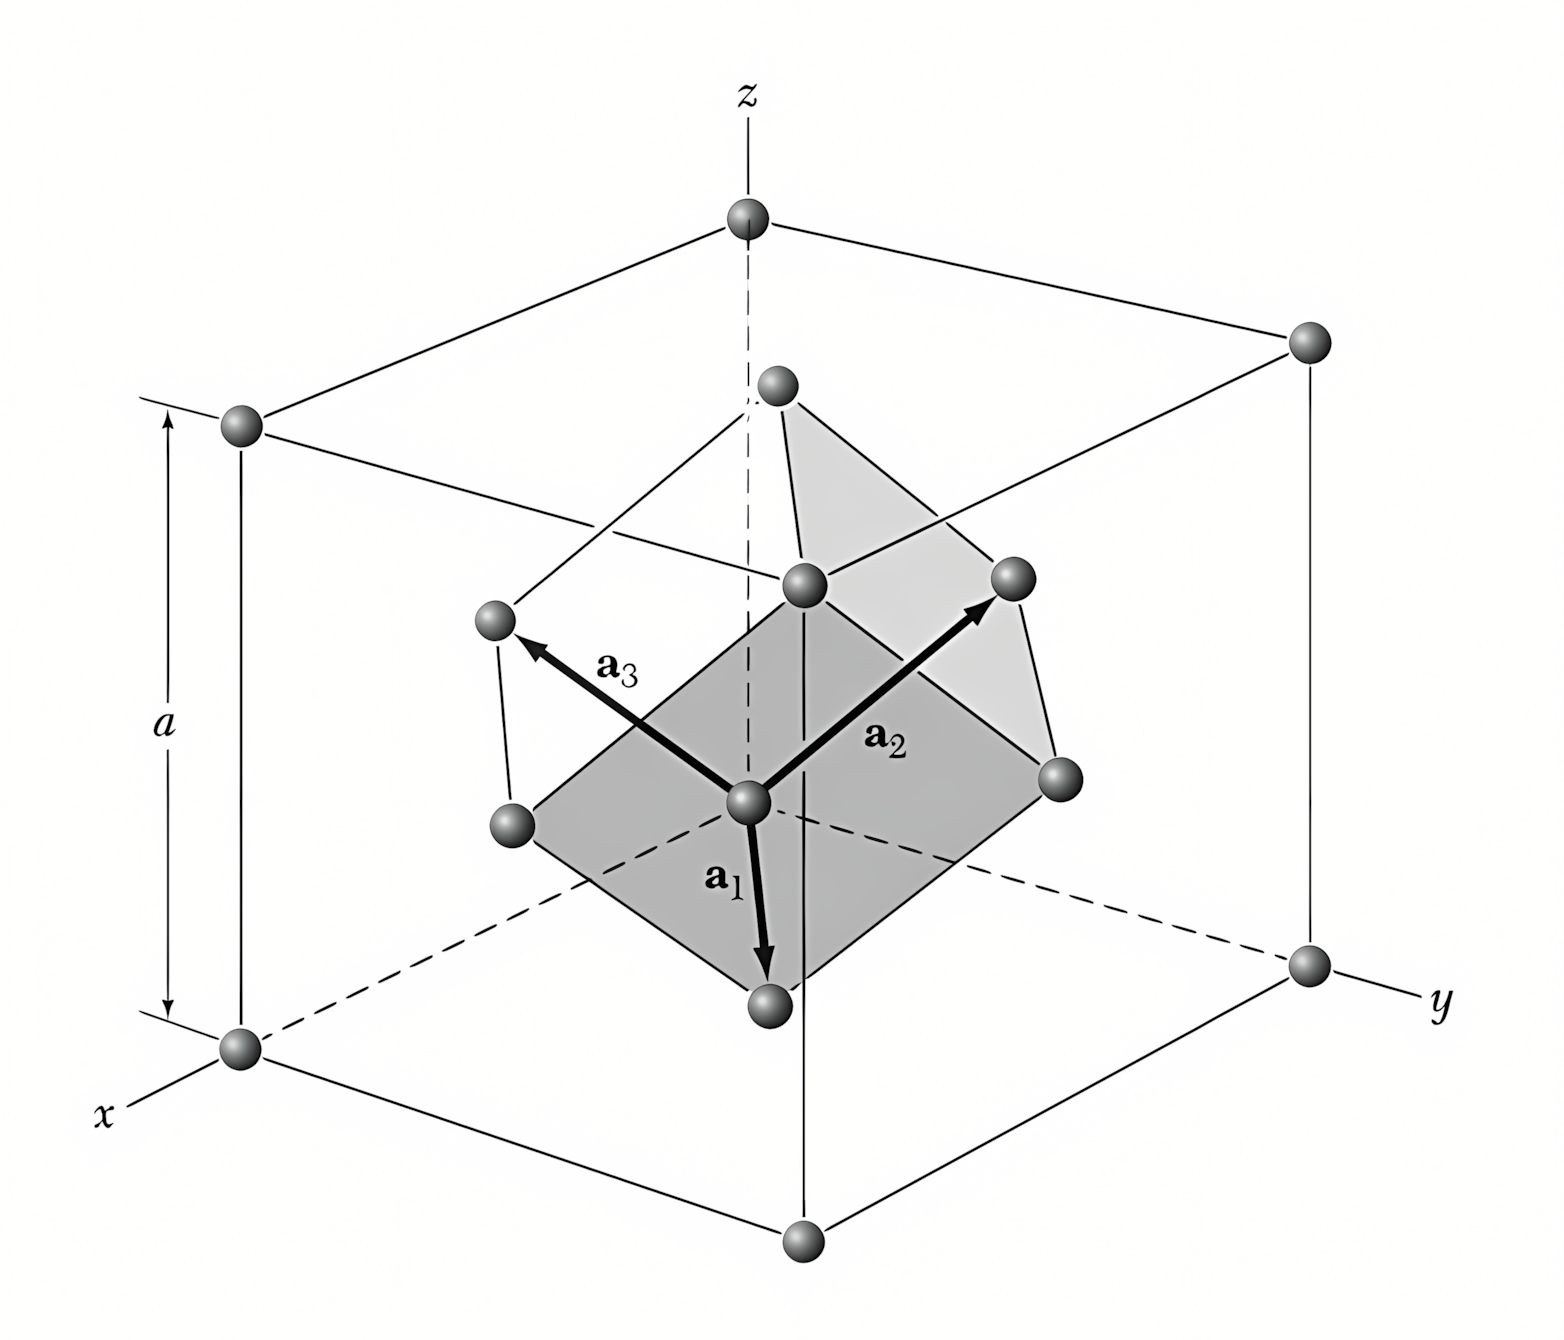
\includegraphics[width=0.7\textwidth]{figures/primitive_cell_fcc.png}
    \caption{Rappresentazione della cella primitiva per il reticolo Cubico a Facce Centrate (FCC).}
    \label{fig:primitive_cell_fcc}
\end{figure}

\textbf{Reticolo Cubico a Facce Centrate (FCC)} \\
Nel sistema FCC, i vettori di base primitivi vengono costruiti assumendo un nodo della cella cartesiana come origine degli assi e tracciando i collegamenti verso i centri di tre facce adiacenti non complanari della cella stessa. Le espressioni che li definiscono sono:
\begin{equation}
\begin{cases}
    \vec{a}'_1 = \frac{1}{2}(\vec{a}_2 + \vec{a}_3) = \frac{1}{2}a(\vec{u}_y + \vec{u}_z) \\
    \vec{a}'_2 = \frac{1}{2}(\vec{a}_3 + \vec{a}_1) = \frac{1}{2}a(\vec{u}_z + \vec{u}_x) \\
    \vec{a}'_3 = \frac{1}{2}(\vec{a}_1 + \vec{a}_2) = \frac{1}{2}a(\vec{u}_x + \vec{u}_y)
\end{cases}
\end{equation}
Questa specifica cella primitiva racchiude al suo interno un solo nodo equivalente. Il suo volume minimo risulta essere un quarto di quello della cella convenzionale:
\begin{equation}
    V_{\text{cell}} = \frac{a^3}{4}
\end{equation}


\begin{figure}[H]
    \centering
    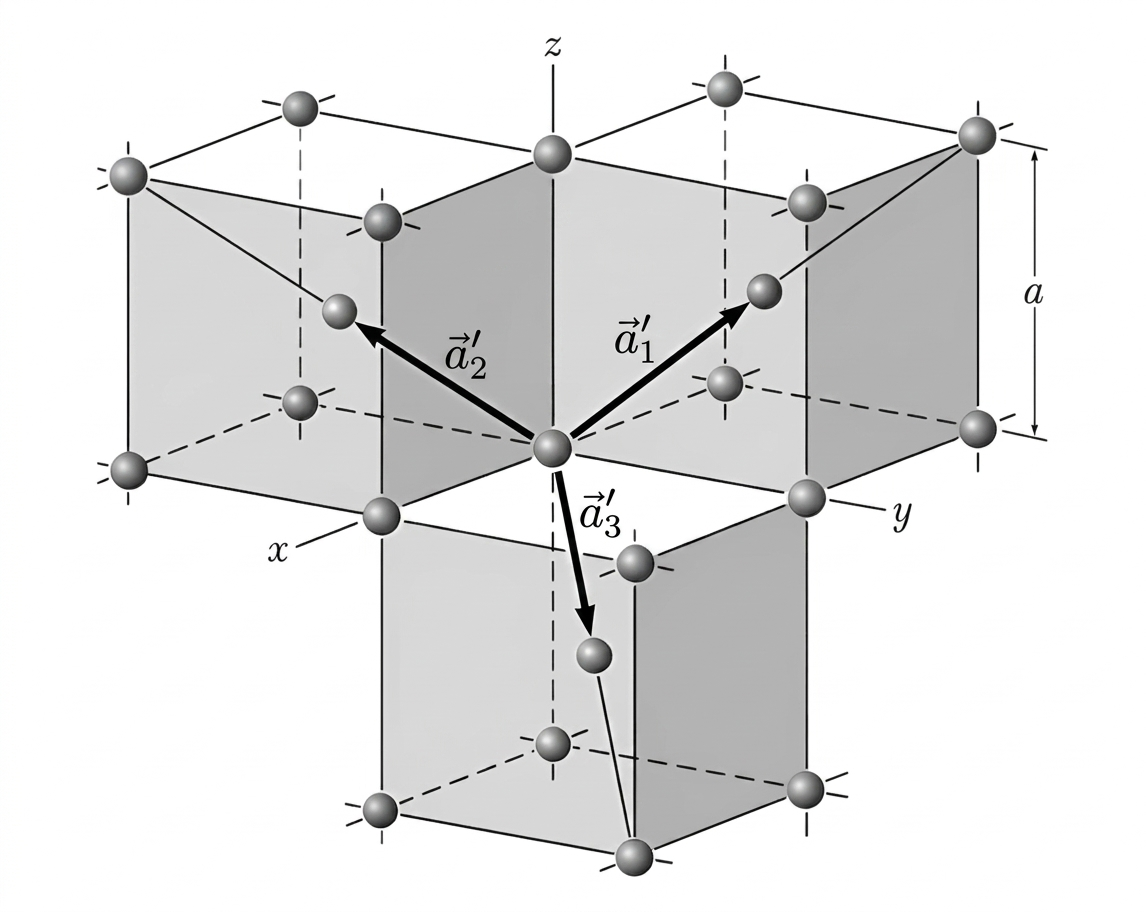
\includegraphics[width=0.7\textwidth]{figures/primitive_cell_bcc.png}
    \caption{Rappresentazione della cella primitiva per il reticolo Cubico a Corpo Centrato (BCC).}
    \label{fig:primitive_cell_bcc}
\end{figure}

\textbf{Reticolo Cubico a Corpo Centrato (BCC)} \\
Per quanto riguarda il sistema BCC, i vettori di base primitivi partono sempre da un vertice della cella cartesiana, ma puntano verso i centri geometrici (dove sono situati i nodi interni) di tre celle cubiche adiacenti. Le relazioni vettoriali sono le seguenti:
\begin{equation}
\begin{cases}
    \vec{a}'_1 = \frac{1}{2}(\vec{a}_2 + \vec{a}_3 - \vec{a}_1) = \frac{1}{2}a(\vec{u}_y + \vec{u}_z - \vec{u}_x) \\
    \vec{a}'_2 = \frac{1}{2}(\vec{a}_3 + \vec{a}_1 - \vec{a}_2) = \frac{1}{2}a(\vec{u}_z + \vec{u}_x - \vec{u}_y) \\
    \vec{a}'_3 = \frac{1}{2}(\vec{a}_1 + \vec{a}_2 - \vec{a}_3) = \frac{1}{2}a(\vec{u}_x + \vec{u}_y - \vec{u}_z)
\end{cases}
\end{equation}
Così come per la struttura FCC, anche questa cella primitiva contiene un solo nodo netto. Il volume calcolato in questo caso corrisponde alla metà del volume della cella cartesiana:
\begin{equation}
    V_{\text{cell}} = \frac{a^3}{2}
\end{equation}

\subsubsection{Periodicità}Fissato un sistema di riferimento basato sui vettori generatori delle traslazioni \( \{\vec{a}_1, \vec{a}_2, \vec{a}_3\} \), è possibile definire un generico vettore del reticolo cristallino come:
\begin{equation}
    \vec{R} = n_1\vec{a}_1 + n_2\vec{a}_2 + n_3\vec{a}_3
\end{equation}

Per il \textbf{Principio di Neumann}, una qualsiasi proprietà fisica \( f \) del materiale (come ad esempio la densità elettronica o l'indice di rifrazione) valutata in una posizione \( \vec{r} \) deve conservarsi invariata a seguito di una traslazione reticolare. Questa invarianza si esprime come:
\begin{equation}
    f(\vec{r}) = f(\vec{r} + \vec{R}) \quad \forall \vec{R}
\end{equation}

Grazie a questa intrinseca periodicità spaziale, la grandezza \( f(\vec{r}) \) può essere scomposta in una serie di Fourier:
\begin{equation}
    f(\vec{r}) = \sum_{\vec{G}} f_{\vec{G}} e^{i \vec{G} \cdot \vec{r}}
\end{equation}
dove i coefficienti dell'espansione sono dati dall'integrale sul volume della cella:
\begin{equation}
    f_{\vec{G}} = \frac{1}{V_{\text{cella}}} \int_{V_{\text{cella}}} f(\vec{r}) e^{-i \vec{G} \cdot \vec{r}} d^3r
\end{equation}

Sostituendo lo sviluppo in serie di Fourier all'interno della condizione di invarianza traslazionale, si deduce che:
\begin{equation}
    \sum_{\vec{G}} f_{\vec{G}} e^{i \vec{G} \cdot \vec{r}} = \sum_{\vec{G}} f_{\vec{G}} e^{i \vec{G} \cdot (\vec{r} + \vec{R})}
\end{equation}
Tale identità risulta valida se e solo se il termine esponenziale aggiuntivo è unitario:
\begin{equation}
    e^{i \vec{G} \cdot \vec{R}} = 1 \iff \vec{G} \cdot \vec{R} = 2\pi m, \quad m \in \mathbb{Z}
\end{equation}

I vettori \( \vec{G} \) che rispettano questa relazione ortogonale formano un luogo di punti nello spazio coniugato che prende il nome di \textbf{reticolo reciproco} (indicato talvolta come reticolo indiretto). 
Esattamente come per il reticolo reale, il reticolo reciproco è descritto da una propria terna di vettori base \( \{\vec{b}_1, \vec{b}_2, \vec{b}_3\} \). Un generico vettore del reticolo reciproco si scrive quindi come combinazione lineare mediante i coefficienti interi \( h, k, l \in \mathbb{Z} \):
\begin{equation}
    \vec{G} = h\vec{b}_1 + k\vec{b}_2 + l\vec{b}_3
\end{equation}

A partire dai vettori base del reticolo diretto \( \{\vec{a}_1, \vec{a}_2, \vec{a}_3\} \), è possibile determinare la terna di vettori \( \{\vec{b}_1, \vec{b}_2, \vec{b}_3\} \) che genera lo spazio del reticolo reciproco. Sfruttando il volume della cella diretta \( V_{\text{cella,RD}} = \vec{a}_1 \cdot \vec{a}_2 \wedge \vec{a}_3 \), tali vettori sono costruiti mediante le seguenti relazioni:

\begin{equation}
\begin{cases}
    \vec{b}_1 = \frac{2\pi}{\vec{a}_1 \cdot \vec{a}_2 \wedge \vec{a}_3} (\vec{a}_2 \wedge \vec{a}_3) = \frac{2\pi}{V_{\text{cella,RD}}} (\vec{a}_2 \wedge \vec{a}_3) \\
    \vec{b}_2 = \frac{2\pi}{\vec{a}_1 \cdot \vec{a}_2 \wedge \vec{a}_3} (\vec{a}_3 \wedge \vec{a}_1) = \frac{2\pi}{V_{\text{cella,RD}}} (\vec{a}_3 \wedge \vec{a}_1) \\
    \vec{b}_3 = \frac{2\pi}{\vec{a}_1 \cdot \vec{a}_2 \wedge \vec{a}_3} (\vec{a}_1 \wedge \vec{a}_2) = \frac{2\pi}{V_{\text{cella,RD}}} (\vec{a}_1 \wedge \vec{a}_2)
\end{cases}
\end{equation}

Questa specifica costruzione matematica assicura il rispetto della condizione di biortogonalità tra le basi dello spazio diretto e di quello reciproco:
\begin{equation}
    \vec{a}_i \cdot \vec{b}_j = 2\pi\delta_{ij}
\end{equation}

In questa nuova base, un generico vettore del reticolo coniugato si esprime come \( \vec{G}_{hkl} = h\vec{b}_1 + k\vec{b}_2 + l\vec{b}_3 \), dove i coefficienti \( (hkl) \) corrispondono esattamente agli indici di Miller dei piani cristallini. Di conseguenza, valutando il prodotto scalare tra \( \vec{G}_{hkl} \) e un vettore di traslazione del reticolo diretto \( \vec{R} = n_1\vec{a}_1 + n_2\vec{a}_2 + n_3\vec{a}_3 \), si ottiene sempre un multiplo intero di \( 2\pi \):
\begin{equation}
    \vec{G} \cdot \vec{R} = 2\pi(n_1h + n_2k + n_3l) = 2\pi m \quad \text{con } m \in \mathbb{Z}
\end{equation}

Risulta evidente come i due reticoli siano intimamente coniugati, implicando che la periodicità dell'uno determini quella dell'altro. Un esempio lampante di questa dualità si osserva nei sistemi cubici: le strutture BCC e FCC sono mutuamente coniugate. Se il materiale presenta un reticolo diretto BCC, il suo spazio reciproco sarà caratterizzato da un reticolo FCC, e viceversa; è perciò essenziale saper gestire il passaggio tra queste due descrizioni.

Così come nello spazio reale, anche nel reticolo reciproco è possibile isolare una cella unitaria, il cui volume si calcola tramite il prodotto misto dei vettori base:
\begin{equation}
    V_{\text{cella,RR}} = \vec{b}_1 \cdot \vec{b}_2 \wedge \vec{b}_3
\end{equation}

L'unità di volume minimo all'interno di questo spazio è definita \textbf{cella primitiva del reticolo reciproco}. Di fondamentale importanza per la trattazione dei materiali cristallini è la \textbf{Zona di Brillouin}, la quale coincide con la cella di Wigner-Seitz costruita per i nodi del reticolo reciproco. Essa geometricamente rappresenta il volume racchiuso dai piani che bisecano ortogonalmente i segmenti congiungenti l'origine con i punti adiacenti del reticolo coniugato.

\lezione{15}{21/05/2026}

È possibile dimostrare la stretta relazione tra il reticolo reciproco e i piani cristallini verificando che il vettore \( \vec{G}_{hkl} \) è ortogonale al piano individuato dagli indici di Miller \( (hkl) \). Per farlo, si definiscono tre vettori generatori giacenti sul piano a partire dalle rispettive intercette con gli assi:
\begin{equation}
\begin{cases}
    \vec{v}_1 = \frac{1}{k}\vec{a}_2 - \frac{1}{l}\vec{a}_3 \\
    \vec{v}_2 = \frac{1}{l}\vec{a}_3 - \frac{1}{h}\vec{a}_1 \\
    \vec{v}_3 = -\frac{1}{h}\vec{a}_1 + \frac{1}{k}\vec{a}_2
\end{cases}
\end{equation}

Calcolando il prodotto scalare tra uno qualsiasi di questi vettori (ad esempio \( \vec{v}_1 \)) e il generico vettore del reticolo reciproco \( \vec{G}_{hkl} = h\vec{b}_1 + k\vec{b}_2 + l\vec{b}_3 \), e sfruttando la proprietà di biortogonalità \( \vec{a}_i \cdot \vec{b}_j = 2\pi\delta_{ij} \), si ottiene:
\begin{equation}
    \vec{v}_1 \cdot \vec{G}_{hkl} = \left( \frac{1}{k}\vec{a}_2 - \frac{1}{l}\vec{a}_3 \right) \cdot (h\vec{b}_1 + k\vec{b}_2 + l\vec{b}_3) = 2\pi \left( \frac{k}{k} - \frac{l}{l} \right) = 0
\end{equation}

Procedendo analogamente per gli altri vettori, i prodotti scalari risultano tutti nulli (\( \vec{v}_2 \cdot \vec{G}_{hkl} = 0 \), \( \vec{v}_3 \cdot \vec{G}_{hkl} = 0 \)). Poiché \( \vec{G}_{hkl} \) è perpendicolare a ogni vettore giacente nel piano, esso rappresenta la normale al piano \( (hkl) \). Il relativo versore normale è dunque:
\begin{equation}
    \hat{n}_{hkl} = \frac{\vec{G}_{hkl}}{|\vec{G}_{hkl}|}
\end{equation}

\textbf{Distanza Interplanare} \\
La distanza \( d_{hkl} \) rispetto all'origine di un piano appartenente alla famiglia \( \{hkl\} \) è valutabile come la proiezione di un generico vettore del reticolo diretto \( \vec{R} = n_1\vec{a}_1 + n_2\vec{a}_2 + n_3\vec{a}_3 \) (che punta a tale piano) lungo la direzione normale:
\begin{equation}
    d_{hkl} = \vec{R} \cdot \hat{n}_{hkl} = \frac{\vec{R} \cdot \vec{G}_{hkl}}{|\vec{G}_{hkl}|}
\end{equation}
Sviluppando il prodotto a numeratore, si ricava un multiplo intero di \( 2\pi \):
\begin{equation}
    \vec{R} \cdot \vec{G}_{hkl} = 2\pi(n_1 h + n_2 k + n_3 l) = 2\pi m \quad \text{con } m \in \mathbb{Z}
\end{equation}
Innestando questo risultato nella formula precedente, la \textbf{distanza minima} tra due piani cristallini adiacenti della medesima famiglia si determina ponendo \( m = 1 \):
\begin{equation}
    d_{hkl,\text{min}} = \frac{2\pi}{|\vec{G}_{hkl}|}
\end{equation}

\textbf{Angolo tra Piani Cristallini} \\
Conoscendo le direzioni normali, è immediato calcolare l'angolo \( \theta \) d'intersezione tra due piani cristallini definiti dagli indici \( (hkl) \) e \( (h'k'l') \). L'angolo scaturisce dalla relazione del prodotto scalare tra i due versori:
\begin{equation}
    \theta = \arccos(\hat{n}_{hkl} \cdot \hat{n}_{h'k'l'}) = \arccos\left( \frac{\vec{G}_{hkl} \cdot \vec{G}_{h'k'l'}}{|\vec{G}_{hkl}| |\vec{G}_{h'k'l'}|} \right)
\end{equation}

In sintesi, il costrutto matematico del reticolo reciproco gode di proprietà geometriche di estrema utilità, in quanto consente di descrivere analiticamente distanze e angoli interplanari, fornendo così la base necessaria per comprendere l'impatto della periodicità strutturale sul comportamento dei solidi cristallini.


\subsection{Diffrazione da raggi X}
Quando un campo elettromagnetico (CEM) incide su un cristallo, è fondamentale conoscere i parametri caratteristici dell'onda incidente, in particolare la lunghezza d'onda \( \lambda \) e la frequenza \( \nu \). Affinché la struttura cristallina possa agire da \textbf{reticolo di diffrazione}, è strettamente necessario che la lunghezza d'onda della radiazione sia comparabile con il parametro di cella \( a \); essi devono cioè possedere il medesimo ordine di grandezza (\( \lambda \approx a \)). 

Nel momento in cui il CEM interagisce con gli atomi del cristallo, l'onda incidente subisce un processo di diffusione. Il fenomeno è concettualmente analogo a quello che avviene in presenza di fenditure, con la differenza che in questo contesto i centri diffusori (gli ostacoli) sono rappresentati dai singoli atomi disposti periodicamente. 

Ogni atomo perturbato fornisce una propria risposta, generando un'onda sferica diffusa. La successiva sovrapposizione spaziale di tutte queste onde secondarie dà luogo a fenomeni di interferenza. La catena logica ineccepibile che descrive il processo fisico è pertanto la seguente:
\textbf{Diffusione} (interazione sui singoli atomi) \( \rightarrow \) \textbf{Interferenza} (sovrapposizione tra le onde diffuse) \( \rightarrow \) \textbf{Generazione della figura di Diffrazione} (il fenomeno macroscopico che viene effettivamente osservato).

Se il modulo del vettore d'onda si conserva inalterato durante il processo, ci si trova in un regime di \textbf{diffusione elastica}. In assenza di perdita o trasferimento di energia, si creano le condizioni ideali per assistere a un'interferenza stabile e ben definita.

Questa dinamica è formalizzabile attraverso il \textbf{Principio di Huygens}: ogni atomo investito dall'onda primaria si comporta come una sorgente puntiforme da cui si genera un'onda di diffusione. Spostandosi a una distanza macroscopica dal cristallo, individuata da un vettore di posizione \( \vec{R}' \), queste molteplici onde secondarie si andranno a combinare linearmente, restituendo il campo elettromagnetico diffratto dal reticolo atomico.

Nel caso specifico in cui si utilizzino raggi X, la risposta del singolo atomo risulta fortemente dipendente dall'energia della radiazione incidente:
\begin{itemize}
    \item Impiegando raggi X a \textbf{bassa energia}, l'onda elettromagnetica interagisce prevalentemente con gli elettroni dei livelli energetici più esterni.
    \item Utilizzando raggi X ad \textbf{alta energia}, la radiazione è sufficientemente penetrante da arrivare a perturbare gli elettroni più vicini al nucleo (elettroni di core).
\end{itemize}

\begin{figure}[htbp]
    \centering
    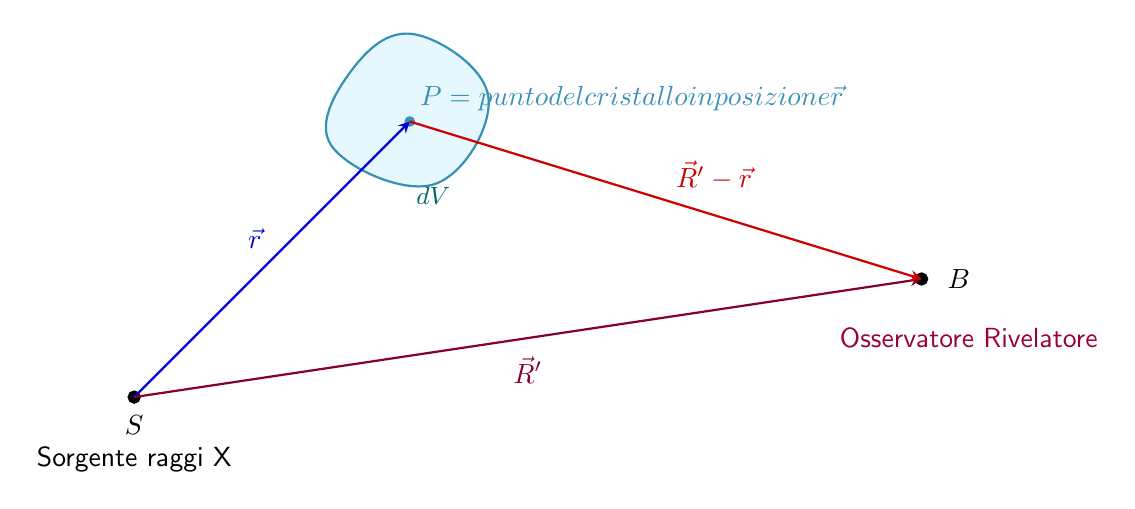
\begin{tikzpicture}[>=stealth, thick, font=\sffamily]

        % Coordinate principali (fondamentale che siano definite prima di usarle)
        \coordinate (S) at (0,0);
        \coordinate (P) at (3.5, 3.5);
        \coordinate (B) at (10, 1.5);

        % --- CRISTALLO ---
        % Le opzioni di lisciatura passate direttamente a plot
        \draw[fill=cyan!10, draw=cyan!70!black] plot[smooth cycle, tension=0.7] coordinates {(2.5, 3.2) (3.8, 2.7) (4.5, 3.8) (3.6, 4.6) (2.8, 4.2)};
        
        % Punto P e volumetto dV
        \filldraw[cyan!70!black] (P) circle (1.5pt) node[above right, text=cyan!70!black] {$P = \text{punto del cristallo in posizione } \vec{r}$};
        \node[right=0.3cm,below = 0.7cm ,font=\small, text=teal!80!black] at (P) {$dV$};

        % --- SORGENTE ---
        \filldraw (S) circle (2pt) node[below=0.1cm] {$S$};
        \node[align=center, below=0.5cm] at (S) {Sorgente raggi X};

        % --- OSSERVATORE / RIVELATORE ---
        \filldraw (B) circle (2pt) node[right=0.2cm] {$B$};
        \node[align= center , right=0.6cm, below=0.5cm,text=purple!80!black] at (B) {Osservatore Rivelatore};

        % --- VETTORI ---
        \draw[->, blue!80!black] (S) -- (P) node[midway, above left] {$\vec{r}$};
        \draw[->, purple!70!black] (S) -- (B) node[midway, below=0.1cm] {$\vec{R}'$};
        \draw[->, red!80!black] (P) -- (B) node[midway, above right] {$\vec{R}' - \vec{r}$};

    \end{tikzpicture}
    \caption{Rappresentazione schematica della geometria di un esperimento di diffrazione da raggi X.}
    \label{fig:xray_diffraction_setup}
\end{figure}


Consideriamo un punto \( P \) all'interno del cristallo, individuato dal vettore posizione \( \vec{r} \). L'interazione con il campo elettromagnetico (CEM) incidente genera in \( P \) una risposta caratterizzata da un'ampiezza \( A_P \), proporzionale alla fase dell'onda incidente:
\begin{equation}
    A_P \propto e^{i \vec{k} \cdot \vec{r}}
\end{equation}
dove \( \vec{k} = \frac{2\pi}{\lambda} \hat{u}_k \) rappresenta il vettore d'onda del CEM incidente.

L'onda diffusa dal punto \( P \) e misurata in un punto di osservazione \( B \) (individuato dal vettore posizione \( \vec{R}' \)) avrà un'ampiezza \( A_B \) che dipende dal cammino ottico percorso dopo l'interazione e dall'attenuazione dell'onda sferica:
\begin{equation}
    A_B \propto A_P \frac{e^{i \vec{k}' \cdot (\vec{R}' - \vec{r})}}{|\vec{R}' - \vec{r}|}
\end{equation}
dove \( \vec{k}' \) è il vettore d'onda diffuso, il quale può differire da \( \vec{k} \) quantomeno nella direzione di propagazione.

L'ampiezza totale osservata, \( A_{B,TOT} \), relativa all'intero cristallo, è data dalla "somma" (ovvero dall'integrazione sul volume) di tutti i singoli contributi generati da ogni centro diffusore. Sostituendo l'espressione di \( A_P \) si ottiene:
\begin{equation}
    A_{B,TOT} \propto \int_{\text{CRISTALLO}} \frac{e^{i \vec{k} \cdot \vec{r}} \cdot e^{i \vec{k}' \cdot (\vec{R}' - \vec{r})}}{|\vec{R}' - \vec{r}|} dV
\end{equation}

Raccogliendo e riordinando i termini all'esponente in funzione della variabile di integrazione \( \vec{r} \):
\begin{equation}
    A_{B,TOT} \propto \int_{\text{CRISTALLO}} e^{-i (\vec{k}' - \vec{k}) \cdot \vec{r}} \underbrace{\frac{e^{i \vec{k}' \cdot \vec{R}'}}{|\vec{R}' - \vec{r}|}}_{:= f(\vec{r})} dV
\end{equation}
A distanze di osservazione macroscopiche, una volta fissate le posizioni (essendo \( |\vec{R}'| \gg |\vec{r}| \)), il termine indicato come \( f(\vec{r}) \) è soggetto a variazioni trascurabili e può essere considerato approssimativamente costante.

Definendo il vettore di trasferimento d'onda (o vettore di scattering) come \( \Delta\vec{k} = \vec{k}' - \vec{k} \), l'integrale si riscrive in forma compatta:
\begin{equation}
    A_{B,TOT} \propto \int_{V_{\text{cristallo}}} e^{-i \Delta\vec{k} \cdot \vec{r}} f(\vec{r}) dV
\end{equation}

Sfruttando la simmetria traslazionale del cristallo, quest'ultimo può essere visto come una singola cella unitaria replicata nello spazio secondo i vettori reticolari \( \vec{R} = n_1\vec{a}_1 + n_2\vec{a}_2 + n_3\vec{a}_3 \). L'integrale sul volume macroscopico può quindi essere ricondotto all'integrale sul volume di una singola cella moltiplicato per il numero totale di celle, \( N_{\text{celle}} \). 
Introducendo esplicitamente la densità elettronica \( n(\vec{r}) \) per quantificare la capacità di diffusione locale, l'ampiezza totale diventa:
\begin{equation}
    A_{B,TOT} \propto N_{\text{celle}} \int_{V_{\text{cella}}} e^{-i \Delta\vec{k} \cdot \vec{r}} f(\vec{r}, \vec{R}') n(\vec{r}) dV
\end{equation}

Affinché si osservi un segnale diffratto macroscopico (\( A_{B,TOT} \neq 0 \)), è necessario analizzare questo contributo elementare. Poiché la diffusione di un campo elettromagnetico a bassa energia è operata prevalentemente dagli elettroni esterni, la parte preponderante dell'intensità è descritta proprio dall'integrale sulla singola cella:
\begin{equation}
    \int_{V_{\text{cella}}} n(\vec{r}) e^{-i \Delta\vec{k} \cdot \vec{r}} f(\vec{r}, \vec{R}') dV
\end{equation}

Valutando il contributo di una generica cella traslata di un vettore reticolare, e sfruttando l'invarianza per traslazione, l'espressione per l'integrale diventa:
\begin{equation}
    I = \int_{V_{\text{cella}}} n(\vec{r} + \vec{R}) e^{-i \Delta\vec{k} \cdot (\vec{r} + \vec{R})} f(\vec{r}, \vec{R}') dV
\end{equation}

In questa formulazione si evidenziano due contributi analitici distinti: il termine esponenziale \( e^{-i \Delta\vec{k} \cdot (\vec{r} + \vec{R})} \), che dipende esplicitamente dalla variazione di fase \( \Delta\vec{k} \), e la funzione \( f(\vec{r}, \vec{R}') \), che funge da termine modulatore dell'intensità.

Applicando il \textbf{Principio di Neumann}, sappiamo che la distribuzione di carica elettronica deve rispettare la medesima periodicità del reticolo spaziale. Pertanto, la densità elettronica è una funzione periodica tale per cui:
\begin{equation}
    n(\vec{r} + \vec{R}) = n(\vec{r}) \quad \forall \vec{R} = n_1\vec{a}_1 + n_2\vec{a}_2 + n_3\vec{a}_3
\end{equation}

Poiché \( \vec{R} \) è un vettore appartenente al cristallo, il Principio di Neumann assicura che il profilo di densità \( n(\vec{r}) \) sia rigorosamente uguale per ogni cella. Di conseguenza, è analiticamente rigoroso e sufficiente calcolare l'integrale di diffusione prendendo come riferimento una cella unitaria qualsiasi del reticolo.
Otteniamo dunque la seguente uguaglianza:
\begin{equation}
    \Rightarrow \int_{V_{\text{cella}}} n(\vec{r}) e^{-i \Delta\vec{k} \cdot \vec{r}} f(\vec{r}, \vec{R}') dV = \int_{V_{\text{cella}}} n(\vec{r}) e^{-i \Delta\vec{k} \cdot (\vec{r} + \vec{R})} f(\vec{r}, \vec{R}') dV
\end{equation}
(passaggio in cui si è usato \( n(\vec{r}) = n(\vec{r} + \vec{R}) \), ovvero l'invarianza traslazionale).

Poiché \( \vec{R} \in \) reticolo diretto generato dai vettori di base \( (\vec{a}_1, \vec{a}_2, \vec{a}_3) \):
\begin{equation}
    \Rightarrow e^{-i \Delta\vec{k} \cdot \vec{R}} = 1 \quad \forall \vec{R}
\end{equation}

Ma tale relazione è intrinsecamente soddisfatta se consideriamo un vettore \( \vec{G} \in \) reticolo reciproco:
\begin{equation}
    \vec{G}_{hkl} = h\vec{b}_1 + k\vec{b}_2 + l\vec{b}_3
\end{equation}
per cui vale:
\begin{equation}
    e^{-i \vec{G}_{hkl} \cdot \vec{R}} = 1 \quad \forall \vec{R}
\end{equation}
data la proprietà di biortogonalità \( \vec{a}_i \cdot \vec{b}_j = 2\pi\delta_{ij} \).

Pertanto, affinché l'ampiezza totale non si annulli (\( A_{B,TOT} \neq 0 \)), deve valere la condizione:
\begin{equation}
    \Delta\vec{k} = \vec{G}_{hkl}
\end{equation}

Come conseguenza della condizione di diffrazione, la variazione del vettore d'onda $\Delta\vec{k}$ può assumere valori appartenenti unicamente a un sottoinsieme discreto di vettori $\vec{G}$. Questi vettori variano a passi interi e costituiscono il \textbf{reticolo reciproco}, il quale è interamente contenuto all'interno del più ampio spazio reciproco.

Considerando che la variazione del vettore d'onda è la differenza tra il vettore d'onda diffuso $\vec{k}'$ e quello incidente $\vec{k}$:
\begin{equation}
    \Delta\vec{k} = \vec{k}' - \vec{k}
\end{equation}
Si possono distinguere due principali regimi di interazione tra il campo elettromagnetico (tipicamente raggi X) e il cristallo:

\begin{itemize}
    \item \textbf{a) Interazione Elastica (Diffusione Elastica):} \\
    È un'interazione tale per cui il modulo del vettore d'onda si conserva inalterato. Non essendoci trasferimento netto di energia, la lunghezza d'onda $\lambda$ rimane costante:
    \begin{equation}
        |\vec{k}| = |\vec{k}'| = \frac{2\pi}{\lambda}
    \end{equation}

    \item \textbf{b) Interazione Inelastica:} \\
    Si verifica quando il modulo del vettore d'onda non si conserva in seguito all'urto con il reticolo:
    \begin{equation}
        |\vec{k}| \neq |\vec{k}'|
    \end{equation}
    In questo scenario, una parte dell'energia della radiazione incidente viene ceduta al cristallo oppure assorbita da esso. Tale "scambio di energia" è tipicamente mediato da specifici canali di interazione interni al materiale, come ad esempio l'eccitazione delle vibrazioni reticolari (fenomeno che verrà analizzato più avanti nel corso).
\end{itemize}


La condizione vettoriale appena ricavata prende il nome di \textbf{Legge di Laue} e governa il fenomeno della diffusione dei raggi X da parte di un cristallo:
\begin{equation}
    \Delta\vec{k} = \vec{G}_{hkl}
\end{equation}
Come diretta conseguenza di questa legge, l'intensità della radiazione diffusa non è distribuita in modo continuo, ma si concentra in "picchi" di intensità distribuiti periodicamente nello spazio; tale distribuzione spaziale riflette specularmente la periodicità del reticolo reciproco, come dimostrato storicamente dall'esperimento di Laue del 1913.

\subsubsection{Equivalenza formulazioni di Bragg e Laue}

In parallelo a questa formulazione, W. L. Bragg propose un approccio fenomenologico alternativo trattando la propagazione dei raggi X attraverso i principi dell'ottica geometrica. Nella visione di Bragg, il fenomeno viene interpretato come un'interferenza costruttiva tra le onde riflesse da \textbf{piani reticolari consecutivi}. 

Definendo \( \theta \) come l'angolo radente compreso tra il vettore d'onda incidente \( \vec{k} \) e il piano reticolare (e non la normale al piano), la condizione per osservare un picco di diffrazione è espressa dalla celebre \textbf{Legge di Bragg}:
\begin{equation}
    2d_{hkl} \sin\theta = m\lambda \quad \text{con } m \in \mathbb{Z}
\end{equation}
dove \( d_{hkl} \) è la distanza interplanare della famiglia di piani considerata. È importante ricordare che questa relazione è formulata nell'ipotesi di diffusione elastica, ovvero quando il modulo del vettore d'onda si conserva (\( |\vec{k}| = |\vec{k}'| \)).

Nonostante le differenze concettuali di partenza, \textbf{le due visioni sono perfettamente equivalenti} e descrivono la medesima fisica:
\begin{itemize}
    \item L'approccio di \textbf{Bragg} ragiona in modo pragmatico sui \textbf{picchi di intensità}, fornendo una relazione scalare (\( 2d_{hkl}\sin\theta = m\lambda \)) che individua in modo diretto la posizione angolare a cui si manifestano.
    \item L'approccio vettoriale di \textbf{Laue} (\( \Delta\vec{k} = \vec{G}_{hkl} \)) risulta invece una trattazione più rigorosa e generale: essa prevede intrinsecamente sia le direzioni in cui si verificano i massimi di intensità, sia le cosiddette estinzioni (ovvero le direzioni in cui l'interferenza è distruttiva).
\end{itemize}


\lezione{16}{21/04/2026}

\textbf{Dimostrazione dell'Equivalenza tra Bragg e Laue} \\
Per dimostrare analiticamente che le due formulazioni descrivono la medesima condizione fisica, è sufficiente partire dal calcolo della differenza di cammino ottico tra le onde diffratte da piani reticolari consecutivi. 

Affinché vi sia interferenza costruttiva, la variazione del percorso ottico \( \Delta s \) deve essere pari a un multiplo intero della lunghezza d'onda \( m\lambda \). Definiamo il vettore reticolare \( \vec{R}_{hkl} \), che congiunge due piani adiacenti muovendosi lungo la direzione normale, come:
\begin{equation}
    \vec{R}_{hkl} = d_{hkl}\hat{n}_{hkl}
\end{equation}

Indicando con \( \hat{u}_{k} \) e \( \hat{u}_{k'} \) i versori che identificano le direzioni di propagazione dell'onda incidente e di quella diffusa rispettivamente, la differenza di cammino ottico si può ricavare per proiezione geometrica:
\begin{equation}
    \Delta s = \vec{R}_{hkl} \cdot (\hat{u}_{k'} - \hat{u}_{k}) = m\lambda
\end{equation}

Moltiplicando ambo i membri dell'equazione per la quantità costante \( \frac{2\pi}{\lambda} \), si ottiene:
\begin{equation}
    \frac{2\pi}{\lambda} (\hat{u}_{k'} - \hat{u}_{k}) \cdot \vec{R}_{hkl} = \frac{2\pi}{\lambda} m\lambda = 2\pi m
\end{equation}

A questo punto si introduce l'ipotesi di \textbf{interazione elastica}, per la quale non vi è perdita di energia e i moduli dei vettori d'onda si conservano: \( |\vec{k}| = |\vec{k}'| = \frac{2\pi}{\lambda} \). Sfruttando questa proprietà, possiamo assorbire il termine \( \frac{2\pi}{\lambda} \) all'interno della parentesi, passando dai versori ai vettori d'onda completi:
\begin{equation}
    (\vec{k}' - \vec{k}) \cdot \vec{R}_{hkl} = 2\pi m
\end{equation}

Sostituendo infine la variazione del vettore d'onda \( \Delta\vec{k} = \vec{k}' - \vec{k} \), l'equazione assume la sua forma più eloquente:
\begin{equation}
    \Delta\vec{k} \cdot \vec{R}_{hkl} = 2\pi m \quad \text{con } m \in \mathbb{Z}
\end{equation}

Questa equazione esprime un concetto fondamentale: il prodotto scalare tra il momento trasferito \( \Delta\vec{k} \) e un vettore del reticolo diretto fornisce sempre un multiplo di \( 2\pi \). Per la definizione stessa di spazio reciproco che abbiamo visto in precedenza, tale relazione risulta verificata se e \textbf{solo se} \( \Delta\vec{k} \) coincide esattamente con un vettore del reticolo reciproco. Abbiamo così ri-ottenuto e dimostrato la validità universale della condizione di Laue:
\begin{equation}
    \Delta\vec{k} = \vec{G}_{hkl}
\end{equation}
\begin{figure}[htbp]
    \centering
    \begin{tikzpicture}[scale=1.5, >=stealth]
    % Parametri geometrici
    \def\d{2}       % Distanza interplanare
    \def\theta{35}  % Angolo radente (theta)

    % Nodi principali
    \coordinate (O) at (0,0);
    \coordinate (B) at (0,-\d);
    
    % Direzioni dei raggi
    \coordinate (InTop) at ({180-\theta}:3.5);
    \coordinate (OutTop) at ({\theta}:3.5);
    \coordinate (InBot) at ($(InTop) + (0,-\d)$);
    \coordinate (OutBot) at ($(OutTop) + (0,-\d)$);

    % Piani reticolari
    \draw[thick] (-3.5, 0) -- (3.5, 0) node[right, font=\Large] {$hkl$};
    \draw[thick] (-3.5, -\d) -- (3.5, -\d);

    % Normale al piano
    \draw[ultra thick] (0, 0) -- (0, 1.5);
    
    % Vettore distanza interplanare d_hkl
    \draw[<->, thick, violet] (0, -0.05) -- (0, -\d+0.05) node[midway, right] {$d_{hkl}$};

    % Raggi sul piano superiore
    \draw[thick, blue, ->] (InTop) -- (O) node[midway, above left, font=\Large] {$\vec{K}$};
    \draw[thick, blue, ->] (O) -- (OutTop) node[midway, above right, font=\Large] {$\vec{K}'$};
    
    % Raggi sul piano inferiore
    \draw[thick, blue, ->] (InBot) -- (B);
    \draw[thick, blue, ->] (B) -- (OutBot);

    % Proiezioni per i fronti d'onda (calcolo esatto)
    \coordinate (ProjIn) at ($(InBot)!(O)!(B)$);
    \coordinate (ProjOut) at ($(B)!(O)!(OutBot)$);

    % Fronti d'onda perpendicolari
    \draw[thick, teal] (O) -- (ProjIn);
    \draw[thick, teal] (O) -- (ProjOut);

    % Differenza di cammino ottico evidenziata (2d sin(theta))
    \draw[ultra thick, teal] (ProjIn) -- (B) node[midway, below left] {$\sim$};
    \draw[ultra thick, teal] (B) -- (ProjOut) node[midway, below right] {$\sim$};

    % Angolo di incidenza theta
    \draw[thick, blue] (-1.2, 0) arc (180:{180-\theta}:1.2) node[midway, left=2pt] {$\theta$};

    % Simboli di angolo retto per i fronti d'onda
    \draw[teal, thin] ($(ProjIn)!0.15!(O)$) -- ($(ProjIn)!0.15!(O)!0.15!(B)$) -- ($(ProjIn)!0.15!(B)$);
    \draw[teal, thin] ($(ProjOut)!0.15!(O)$) -- ($(ProjOut)!0.15!(O)!0.15!(B)$) -- ($(ProjOut)!0.15!(B)$);

\end{tikzpicture}
    \caption{Rappresentazione schematica dell'equivalenza tra Bragg e Laue.}
    \label{fig:bragg_laue_equivalence}
\end{figure}

Partendo invece dalla condizione di Laue, la la dimostrazine la si può ottenere per via geometrica. Considerando la diffusione elastica, i vettori d'onda incidente \( \vec{k} \) e diffuso \( \vec{k}' \) formano un rombo con il vettore momento trasferito \( \Delta\vec{k} \). Conservandosi il modulo, abbiamo:
\begin{equation}
    k = k' = \frac{2\pi}{\lambda}
\end{equation}

Dalla trigonometria della figura, sapendo che \( \theta \) è l'angolo radente rispetto al piano, la lunghezza del vettore differenza risulta pari a:
\begin{equation}
    |\Delta\vec{k}| = 2k \sin\theta
\end{equation}

Imponendo la condizione di diffrazione di Laue in termini di moduli, ovvero \( |\Delta\vec{k}| = |\vec{G}_{hkl}| \), e richiamando la relazione che lega il vettore reciproco alla distanza interplanare \( d_{hkl} = \frac{2\pi m}{|\vec{G}_{hkl}|} \rightarrow |\vec{G}_{hkl}| = \frac{2\pi m}{d_{hkl}} \), possiamo eguagliare le due quantità:
\begin{equation}
    2k \sin\theta = \frac{2\pi m}{d_{hkl}}
\end{equation}

Sostituendo l'espressione di \( k \) all'interno di questa uguaglianza, otteniamo:
\begin{equation}
    2 \left( \frac{2\pi}{\lambda} \right) \sin\theta = \frac{2\pi m}{d_{hkl}}
\end{equation}

Semplificando il termine \( 2\pi \) presente in entrambi i membri della relazione e riorganizzando i fattori, si perviene in modo diretto alla Condizione di Bragg:
\begin{equation}
    2d_{hkl} \sin\theta = m\lambda
\end{equation}

\begin{attention}
    Nonostante questo passaggio algebrico mostri la stretta connessione tra le due leggi, non si tratta di un'equivalenza matematica perfetta a tutti i livelli. 
    Entrambi gli approcci (Bragg e Laue) consentono di individuare con successo le posizioni angolari in cui si verificano i massimi di intensità.
    Tuttavia, la formulazione vettoriale di Laue risulta essere più completa e ricca di informazioni: essa è in grado di prevedere le cosiddette \textbf{estinzioni sistematiche}, 
    ovvero specifiche configurazioni di diffrazione in cui si verifica un'interferenza completamente distruttiva, facendo "scomparire" picchi di intensità che, limitandosi alla sola visione geometrica di Bragg, dovrebbero teoricamente manifestarsi.

\end{attention}

\subsubsection{Quantificazione della diffrazione}
Riprendendo l'espressione dell'ampiezza di diffusione totale, essa è proporzionale al numero di celle e all'integrale sul volume della singola cella:
\begin{equation}
    A \propto N_{\text{celle}} \int_{V_{\text{cella}}} n(\vec{r}) e^{-i \Delta\vec{k} \cdot \vec{r}} f(\vec{r}, \vec{R}') d^3r
\end{equation}
dove \( n(\vec{r}) \) rappresenta la densità elettronica locale.

Il termine \( f(\vec{r}, \vec{R}') \), che descrive l'ampiezza dell'onda sferica diffusa, è inversamente proporzionale alla distanza tra il punto di scattering e il punto di osservazione:
\begin{equation}
    f(\vec{r}, \vec{R}') \propto \frac{1}{|\vec{R}' - \vec{r}|}
\end{equation}
Dal momento che il rivelatore è posizionato a distanze macroscopiche rispetto alle dimensioni atomiche (\( |\vec{R}'| \gg |\vec{r}| \)), questo termine varia in modo del tutto trascurabile all'interno della cella unitaria. Pertanto, può essere considerato approssimativamente costante ai fini dell'integrazione.

Sotto questa approssimazione, il \textbf{fattore dominante} che governa l'intensità e la modulazione del segnale diffratto è dato esclusivamente dall'integrale della densità di carica pesato per il fattore di fase:
\begin{equation}
    \int_{V_{\text{cella}}} n(\vec{r}) e^{-i \Delta\vec{k} \cdot \vec{r}} d^3r
\end{equation}

Fisicamente, all'interno di ogni singola cella, sono gli elettroni a subire i processi di scattering e a generare il pattern di diffrazione. Per calcolare esplicitamente questo integrale per un materiale reale, è necessario prima identificare la base associata al reticolo, ovvero determinare il numero minimo di atomi abbinati alla cella unitaria in grado di rappresentare in modo completo la struttura del cristallo.

Consideriamo ad esempio un reticolo cubico a corpo centrato (BCC): pur presentando atomi su tutti gli 8 vertici e uno al centro, la sua base è costituita da soli $s = 2$ atomi (convenzionalmente, un atomo nell'origine e uno posizionato al centro del cubo). Traslando questa coppia di atomi lungo i nodi del reticolo di Bravais associato, si coprono perfettamente tutti i vertici e tutti i centri. Una scelta errata della base, ad esempio prendendo due vertici, porterebbe a sovrastimare alcune posizioni a causa delle condivisioni e a omettere del tutto gli atomi centrali.

Denotando con $\vec{d}_j$ il vettore posizione del $j$-esimo atomo della base rispetto all'origine della cella unitaria, la densità elettronica totale $n(\vec{r})$ all'interno della cella può essere espressa come la somma dei contributi locali $n_j$ dei singoli $s$ atomi:
\begin{equation}
    n(\vec{r}) = \sum_{j=1}^{s} n_j(\vec{r} - \vec{d}_j)
\end{equation}

Sostituendo questa scomposizione all'interno dell'integrale che definisce il fattore dominante per l'ampiezza di diffusione, otteniamo:
\begin{equation}
    I = \int_{V_{\text{cella}}} n(\vec{r}) e^{-i \Delta\vec{k} \cdot \vec{r}} d^3r = \sum_{j=1}^{s} \int_{V_{\text{cella}}} n_j(\vec{r} - \vec{d}_j) e^{-i \Delta\vec{k} \cdot \vec{r}} d^3r
\end{equation}

Per agevolare la risoluzione, si opera un cambio di variabile definendo un vettore posizione locale per ogni atomo: $\vec{\rho} = \vec{r} - \vec{d}_j$, da cui banalmente $\vec{r} = \vec{\rho} + \vec{d}_j$. Riscrivendo l'esponenziale per tenere conto del cambio di coordinate e portando fuori dall'integrale i termini indipendenti dalla variabile d'integrazione, la formula diviene:
\begin{equation}
    I = \sum_{j=1}^{s} e^{-i \Delta\vec{k} \cdot \vec{d}_j} \int_{V_{\text{cella}}} n_j(\vec{\rho}) e^{-i \Delta\vec{k} \cdot \vec{\rho}} d^3\rho
\end{equation}

Analizzando quest'ultima espressione, l'integrale al suo interno dipende unicamente dalla distribuzione di densità elettronica locale $n_j(\vec{\rho})$ dell'atomo $j$-esimo. 
Il termine appena individuato prende il nome di \textbf{fattore di forma} ed è definito analiticamente come:
\begin{equation}
    f_j = \int_{\text{atomo } j\text{-esimo}} n_j(\vec{\rho}) e^{-i \Delta\vec{k} \cdot \vec{\rho}} d^3\rho
\end{equation}
Questo parametro quantifica la capacità di scattering del singolo atomo. Essendo legato alla densità elettronica, è una grandezza specifica per ogni elemento chimico e risulta approssimativamente proporzionale al suo numero atomico (\( f_j \propto Z_j \)). Naturalmente, se il fattore di forma di uno specifico centro diffusore fosse nullo (\( f_j = 0 \)), esso non genererebbe alcuna diffrazione, contribuendo solo all'estinzione del segnale.

Sostituendo il fattore di forma nell'equazione generale che descrive l'ampiezza diffusa dalla cella unitaria, si ottiene:
\begin{equation}
    I = \sum_{j=1}^{s} f_j e^{-i \Delta\vec{k} \cdot \vec{d}_j}
\end{equation}

Sapendo che i picchi di diffrazione macroscopici si osservano unicamente quando è soddisfatta la condizione di Laue (\( \Delta\vec{k} = \vec{G}_{hkl} \)), possiamo valutare questa quantità proprio in corrispondenza dei nodi del reticolo reciproco. Questa valutazione definisce il \textbf{fattore di struttura} \( S_{hkl} \):
\begin{equation}
    S_{hkl} = I \Big|_{\Delta\vec{k} = \vec{G}_{hkl}} = \sum_{j=1}^{s} f_j e^{-i \vec{G}_{hkl} \cdot \vec{d}_j}
\end{equation}

Il fattore di struttura è la quantità fisica fondamentale che determina l'intensità (e quindi la presenza o l'assenza) dei picchi di diffrazione previsti geometricamente dal reticolo. Per verificare se in corrispondenza di un set di indici di Miller \( (hkl) \) comparirà effettivamente un picco, dobbiamo analizzare il risultato di questa sommatoria:
\begin{itemize}
    \item \textbf{Se} \( S_{hkl} = 0 \): i contributi di fase dei vari atomi della base si elidono a vicenda. In questo caso si verifica un'interferenza totalmente distruttiva e si parla di \textbf{estinzione} (il picco previsto dalla legge di Bragg scompare).
    \item \textbf{Se} \( S_{hkl} \neq 0 \): i contributi non si annullano, si ha interferenza costruttiva e si osserva un netto picco di \textbf{diffrazione}.
\end{itemize}


\begin{exercise}
    
\textbf{da Esame} \\
Si consideri un cristallo di Rame (Cu) caratterizzato da una struttura FCC. Dai dati di letteratura si ha:
\begin{itemize}
    \item Massa molare: \( P_{Cu} = 63.55 \, \text{g/mol} \)
    \item Densità di massa: \( \rho_{Cu} = 8.9 \, \text{g/cm}^3 \)
\end{itemize}

\textbf{Richieste:}
\begin{enumerate}
    \item[a)] Calcolare il parametro di cella \( a \) (lato del cubo della cella cartesiana).
    \item[b)] Calcolare la distanza interplanare \( d_{hkl} \) per la famiglia di piani (220).
    \item[c)] Calcolare l'angolo \( \theta \) compreso tra i piani (220) e (211).
\end{enumerate}


\begin{solution}
    \textbf{a)}
Iniziamo con la definizione geometrica della \textbf{cella cartesiana} (è buona norma specificare sempre i vettori di base in funzione della cella scelta). Fissata una terna di versori ortonormali \( \{\hat{x}, \hat{y}, \hat{z}\} \) e indicato con \( a \) il parametro di cella, i vettori generatori del reticolo diretto sono:
\begin{equation}
\begin{cases}
    \vec{a}_1 = a\hat{x} \\
    \vec{a}_2 = a\hat{y} \\
    \vec{a}_3 = a\hat{z}
\end{cases}
\end{equation}

Per definizione, il volume della cella cartesiana si ottiene attraverso il prodotto misto dei vettori base:
\begin{equation}
    V_{\text{cella}} = \vec{a}_1 \cdot (\vec{a}_2 \wedge \vec{a}_3) = a\hat{x} \cdot (a\hat{y} \wedge a\hat{z}) = a^3
\end{equation}

Introduciamo il concetto di \textbf{densità atomica} (\( \rho_{\text{atomica}} \)), che esprime il numero di atomi racchiusi nell'unità di volume:
\begin{equation}
    \rho_{\text{atomica}} = \frac{n^\circ \text{ atomi}}{V_{\text{cella}}}
\end{equation}

Per il reticolo Cubico a Facce Centrate (FCC) in esame, il numero di atomi equivalenti per cella unitaria si calcola sommando i contributi dei nodi condivisi:
\begin{equation}
    n^\circ \text{ atomi}_{\text{FCC}} = \left( \frac{1}{8} \cdot 8 \text{ vertici} \right) + \left( \frac{1}{2} \cdot 6 \text{ facce} \right) = 1 + 3 = 4
\end{equation}
Ne consegue che la densità atomica in funzione del parametro incognito risulta essere:
\begin{equation}
    \rho_{\text{atomica}} = \frac{4}{a^3}
\end{equation}

Trattandosi di un cristallo monoelementale di Cu, la \textbf{densità di massa macroscopica} (\( \rho_{\text{massa}} \)) si ricava semplicemente moltiplicando la massa di un singolo atomo (\( m_{Cu} \)) per la densità atomica. Sapendo che la massa di un singolo atomo è pari al rapporto tra la massa molare \( P_{Cu} \) e il numero di Avogadro \( N_A \):
\begin{equation}
    \rho_{\text{massa}} = m_{Cu} \cdot \rho_{\text{atomica}} \quad \Rightarrow \quad \rho_{\text{massa}} = \frac{P_{Cu}}{N_A} \cdot \rho_{\text{atomica}}
\end{equation}

Sostituendo l'espressione analitica della densità atomica, otteniamo l'equazione finale per la densità di massa, da cui si potrà estrarre il parametro \( a \):
\begin{equation}
    \rho_{\text{massa}} = 8.9 \, \text{g/cm}^3 = \frac{P_{Cu}}{N_A} \cdot \frac{4}{a^3} \implies a \simeq 0.36 \, \text{nm}
\end{equation}
L'ordine di grandezza  di \(10^{-10} \, \text{m}\) è quello che ci aspettiamo.

\textbf{b)} 
La distanza interplanare (intesa come distanza minima tra i piani della famiglia) è legata al modulo del vettore del reticolo reciproco corrispondente dalla relazione:
\begin{equation}
    d_{220} = \frac{2\pi}{|\vec{G}_{220}|}
\end{equation}

Per ricavare tale vettore, è necessario prima esplicitare i vettori di base del reticolo reciproco $\{\vec{b}_1, \vec{b}_2, \vec{b}_3\}$, coniugati alla base del reticolo diretto $\{\vec{a}_1, \vec{a}_2, \vec{a}_3\}$. Sapendo dal punto precedente che $V_{\text{cella}} = a^3$:
\begin{equation}
\begin{cases}
    \vec{b}_1 = \frac{2\pi}{V_{\text{cella}}} (\vec{a}_2 \wedge \vec{a}_3) = \frac{2\pi}{a^3} (a\hat{y} \wedge a\hat{z}) = \frac{2\pi}{a} \hat{x} \\
    \vec{b}_2 = \frac{2\pi}{V_{\text{cella}}} (\vec{a}_3 \wedge \vec{a}_1) = \frac{2\pi}{a^3} (a\hat{z} \wedge a\hat{x}) = \frac{2\pi}{a} \hat{y} \\
    \vec{b}_3 = \frac{2\pi}{V_{\text{cella}}} (\vec{a}_1 \wedge \vec{a}_2) = \frac{2\pi}{a^3} (a\hat{x} \wedge a\hat{y}) = \frac{2\pi}{a} \hat{z}
\end{cases}
\end{equation}

Possiamo ora costruire il vettore reciproco $\vec{G}_{220}$ tramite la combinazione lineare indicata dagli indici di Miller:
\begin{equation}
    \vec{G}_{220} = 2\vec{b}_1 + 2\vec{b}_2 + 0\vec{b}_3 = 2 \cdot \frac{2\pi}{a} (\hat{x} + \hat{y})
\end{equation}

Il modulo di questo vettore risulta essere:
\begin{equation}
    |\vec{G}_{220}| = \frac{4\pi}{a} \sqrt{1^2 + 1^2} = 4\sqrt{2} \frac{\pi}{a}
\end{equation}

Sostituendo il modulo appena trovato nella formula per la distanza interplanare:
\begin{equation}
    d_{220} = \frac{2\pi}{\frac{4\pi\sqrt{2}}{a}} = a \frac{\sqrt{2}}{4}
\end{equation}
Calcolando numericamente (sfruttando il valore di $a$ precedentemente dedotto), si ottiene un valore di circa:
\begin{equation}
    d_{220} \approx 0.127 \, \text{nm}
\end{equation}

\textbf{c)}
Per poter calcolare l'angolo richiesto, è necessario ricavare prima il vettore reciproco relativo alla seconda famiglia di piani $\vec{G}_{211}$ e il suo rispettivo modulo, procedendo in modo analogo:
\begin{equation}
    \vec{G}_{211} = 2\vec{b}_1 + 1\vec{b}_2 + 1\vec{b}_3 = \frac{2\pi}{a} (2\hat{x} + \hat{y} + \hat{z})
\end{equation}

Il calcolo del modulo fornisce:
\begin{equation}
    |\vec{G}_{211}| = \left( \frac{4\pi^2}{a^2} (2^2 + 1^2 + 1^2) \right)^{1/2} = \left( \frac{24\pi^2}{a^2} \right)^{1/2} = 2\sqrt{6} \frac{\pi}{a}
\end{equation}

Sfruttando la relazione di ortogonalità $\vec{b}_i \cdot \vec{b}_j = \delta_{ij} \frac{4\pi^2}{a^2}$, l'angolo $\theta$ si calcola in un unico passaggio tramite il prodotto scalare tra i vettori del reticolo reciproco $\vec{G}_{220}$ e $\vec{G}_{211}$:

\begin{equation}
    \theta = \arccos \left( \frac{\vec{G}_{220} \cdot \vec{G}_{211}}{|\vec{G}_{220}| |\vec{G}_{211}|} \right) = \arccos \left( \frac{ \frac{4\pi^2}{a^2} (2\cdot 2 + 2\cdot 1 + 0\cdot 1) }{ \left( \frac{2\pi}{a} \sqrt{8} \right) \left( \frac{2\pi}{a} \sqrt{6} \right) } \right)
\end{equation}

Semplificando direttamente i termini comuni a numeratore e denominatore:

\begin{equation}
    \theta = \arccos \left( \frac{24}{8\sqrt{12}} \right) = \arccos \left( \frac{3}{2\sqrt{3}} \right) = \arccos \left( \frac{\sqrt{3}}{2} \right) = 30^\circ
\end{equation}

\end{solution}
\end{exercise}


\begin{note}{Fattore di Struttura ed Estinzioni nel reticolo FCC}{}
Valutiamo quali sono le estinzioni sistematiche attese per il reticolo FCC calcolando il fattore di struttura rispetto alla cella cartesiana. 

Definiamo innanzitutto i 4 atomi di base $\{\vec{d}_j\}$ che caratterizzano la cella unitaria del cristallo. Ricordando i vettori primitivi precedentemente ricavati, le posizioni sono:
\begin{equation}
\begin{cases}
    \vec{d}_1 = \vec{0} & \text{(atomo nell'origine)} \\
    \vec{d}_2 = a(0, \frac{1}{2}, \frac{1}{2}) = \frac{\vec{a}_2 + \vec{a}_3}{2} & \text{(vettore primitivo } \vec{a}'_1 \text{)} \\
    \vec{d}_3 = a(\frac{1}{2}, 0, \frac{1}{2}) = \frac{\vec{a}_1 + \vec{a}_3}{2} & \text{(vettore primitivo } \vec{a}'_2 \text{)} \\
    \vec{d}_4 = a(\frac{1}{2}, \frac{1}{2}, 0) = \frac{\vec{a}_1 + \vec{a}_2}{2} & \text{(vettore primitivo } \vec{a}'_3 \text{)}
\end{cases}
\end{equation}

Costruiamo la sommatoria del fattore di struttura sui 4 atomi, espandendo i termini. Trattandosi di un cristallo monoelementale, i fattori di forma atomici sono identici per tutti i siti ($f_j \approx f_Z$):
\begin{equation}
    S_{hkl} = \sum_{j=1}^{4} f_j e^{-i\vec{G}_{hkl} \cdot \vec{d}_j} = f_Z \left( e^{-i\vec{G}_{hkl} \cdot \vec{d}_1} + e^{-i\vec{G}_{hkl} \cdot \vec{d}_2} + e^{-i\vec{G}_{hkl} \cdot \vec{d}_3} + e^{-i\vec{G}_{hkl} \cdot \vec{d}_4} \right)
\end{equation}

Esplicitando i prodotti scalari con il vettore del reticolo reciproco $\vec{G}_{hkl} = \frac{2\pi}{a}(h\hat{x} + k\hat{y} + l\hat{z})$ e semplificando i termini comuni $\frac{2\pi}{a}$ con $\frac{a}{2}$, otteniamo direttamente le fasi in funzione degli indici di Miller:
\begin{equation}
    S_{hkl} = f_Z \left\{ 1 + e^{-i\pi(k+l)} + e^{-i\pi(h+l)} + e^{-i\pi(h+k)} \right\}
\end{equation}

Analizzando gli esponenti di questa equazione finale, si deducono le regole di selezione dei picchi di diffrazione per il reticolo FCC:
\begin{itemize}
    \item $S_{hkl} = \text{max}$: se gli indici $(h,k,l)$ sono \textbf{tutti pari o tutti dispari}. In questo caso gli esponenziali valgono tutti $+1$, l'interferenza è totalmente costruttiva e si osserva il picco.
    \item $S_{hkl} = 0$: se si hanno \textbf{indici misti} (es. un indice pari e gli altri dispari, o viceversa). In questo caso le fasi si elidono causando interferenza distruttiva; la geometria della cella "spegne" il picco di diffrazione generando le \textbf{ESTINZIONI}.
\end{itemize}
\end{note}


\textbf{Atomi a più elettroni} \\
Per descrivere sistemi complessi a \( n \) elettroni, l'Hamiltoniana completa assume la forma:
\begin{equation}
    H = T + V_{eN} + V_{NN} + V_{ee} + \Delta H_{\text{correz.}}
\end{equation}
L'equazione di Schrödinger stazionaria associata è \( H\Psi_E = E\Psi_E \), dove la funzione d'onda complessiva dipende dalle coordinate spaziali di tutti gli elettroni e dei nuclei, oltre che dallo spin:
\begin{equation}
    \Psi_E = \Psi_E(\{ \vec{r}_{e,i} \}_{i=1,\dots,N_e}, \{ \vec{R}_{N,j} \}_{j=1,\dots,N_N}, \text{SPIN})
\end{equation}
Affinché sia fisicamente accettabile, tale funzione d'onda \( \Psi_E \) deve essere \textbf{antisimmetrica} per rispettare il Principio di esclusione di Pauli.

\textbf{Approccio a componenti} \\
Un approccio alternativo consiste nell'osservare la risposta del sistema scomponendo l'Hamiltoniana nei suoi diversi contributi fisici:
\begin{equation}
    H = \underbrace{H_N}_{\text{contrib. nucleare}} + \underbrace{H_{e,\text{valenza}}}_{\text{elettroni esterni}} + \underbrace{H_{e,\text{core}}}_{\text{elettroni interni}} + \Delta H_{\text{residuo}}
\end{equation}

Analizzando il ruolo delle diverse componenti elettroniche:
\begin{itemize}
    \item \textbf{Elettroni di valenza} (\( H_{e,\text{valenza}} \)): sono gli elettroni più esterni e risentono in misura minore dell'attrazione nucleare. Di conseguenza, possono allontanarsi dal nucleo padre e "giocare" (interagire) con l'ambiente circostante. L'interazione con un campo elettromagnetico (CEM) ordinario dipende prevalentemente dalla loro dinamica.
    \item \textbf{Elettroni di core} (\( H_{e,\text{core}} \)): sono gli elettroni dei gusci più profondi, i quali risultano fortemente localizzati in prossimità del nucleo.
\end{itemize}

Mentre le interazioni ottiche convenzionali coinvolgono primariamente gli elettroni di valenza, l'utilizzo dei \textbf{raggi X} cambia lo scenario. Essendo radiazioni estremamente energetiche (da \( 100 \, \text{eV} \) fino a \( 10^5 \, \text{eV} \)), i raggi X sono in grado di penetrare nel materiale e intervenire direttamente sugli elettroni di core.

A seconda della specifica categoria di proprietà fisiche che si intende studiare, ci si può concentrare solo su una determinata porzione dell'Hamiltoniana \( H \) e della funzione d'onda \( \Psi \); il resto dei gradi di libertà viene trattato in modo approssimato come un "contributo medio" di fondo, concettualmente in linea con l'approssimazione di Hartree-Fock.

\textbf{Periodicità del potenziale} \\
Focalizzando l'attenzione sull'Hamiltoniana di un sistema cristallino, si evidenzia una fondamentale proprietà di simmetria:
\begin{equation}
    H = T + V_{ee} + V_{eN} + V_{NN}
\end{equation}
I termini di potenziale \( V_{eN} \) (interazione elettrone-nucleo) e \( V_{NN} \) (interazione nucleo-nucleo) sono \textbf{periodici} in virtù della rigorosa disposizione degli atomi nel reticolo spaziale, definito dai vettori di traslazione \( \vec{R} = n_1\vec{a}_1 + n_2\vec{a}_2 + n_3\vec{a}_3 \). Come diretta conseguenza di questa periodicità del potenziale imposto dalla struttura, la funzione d'onda \( \Psi_E \) che descrive gli elettroni nel cristallo andrà inevitabilmente a "ereditare" tale periodicità.


